% Options for packages loaded elsewhere
\PassOptionsToPackage{unicode}{hyperref}
\PassOptionsToPackage{hyphens}{url}
%
\documentclass[
  man,floatsintext]{apa6}
\usepackage{amsmath,amssymb}
\usepackage{lmodern}
\usepackage{iftex}
\ifPDFTeX
  \usepackage[T1]{fontenc}
  \usepackage[utf8]{inputenc}
  \usepackage{textcomp} % provide euro and other symbols
\else % if luatex or xetex
  \usepackage{unicode-math}
  \defaultfontfeatures{Scale=MatchLowercase}
  \defaultfontfeatures[\rmfamily]{Ligatures=TeX,Scale=1}
\fi
% Use upquote if available, for straight quotes in verbatim environments
\IfFileExists{upquote.sty}{\usepackage{upquote}}{}
\IfFileExists{microtype.sty}{% use microtype if available
  \usepackage[]{microtype}
  \UseMicrotypeSet[protrusion]{basicmath} % disable protrusion for tt fonts
}{}
\makeatletter
\@ifundefined{KOMAClassName}{% if non-KOMA class
  \IfFileExists{parskip.sty}{%
    \usepackage{parskip}
  }{% else
    \setlength{\parindent}{0pt}
    \setlength{\parskip}{6pt plus 2pt minus 1pt}}
}{% if KOMA class
  \KOMAoptions{parskip=half}}
\makeatother
\usepackage{xcolor}
\usepackage{graphicx}
\makeatletter
\def\maxwidth{\ifdim\Gin@nat@width>\linewidth\linewidth\else\Gin@nat@width\fi}
\def\maxheight{\ifdim\Gin@nat@height>\textheight\textheight\else\Gin@nat@height\fi}
\makeatother
% Scale images if necessary, so that they will not overflow the page
% margins by default, and it is still possible to overwrite the defaults
% using explicit options in \includegraphics[width, height, ...]{}
\setkeys{Gin}{width=\maxwidth,height=\maxheight,keepaspectratio}
% Set default figure placement to htbp
\makeatletter
\def\fps@figure{htbp}
\makeatother
\setlength{\emergencystretch}{3em} % prevent overfull lines
\providecommand{\tightlist}{%
  \setlength{\itemsep}{0pt}\setlength{\parskip}{0pt}}
\setcounter{secnumdepth}{-\maxdimen} % remove section numbering
% Make \paragraph and \subparagraph free-standing
\ifx\paragraph\undefined\else
  \let\oldparagraph\paragraph
  \renewcommand{\paragraph}[1]{\oldparagraph{#1}\mbox{}}
\fi
\ifx\subparagraph\undefined\else
  \let\oldsubparagraph\subparagraph
  \renewcommand{\subparagraph}[1]{\oldsubparagraph{#1}\mbox{}}
\fi
\newlength{\cslhangindent}
\setlength{\cslhangindent}{1.5em}
\newlength{\csllabelwidth}
\setlength{\csllabelwidth}{3em}
\newlength{\cslentryspacingunit} % times entry-spacing
\setlength{\cslentryspacingunit}{\parskip}
\newenvironment{CSLReferences}[2] % #1 hanging-ident, #2 entry spacing
 {% don't indent paragraphs
  \setlength{\parindent}{0pt}
  % turn on hanging indent if param 1 is 1
  \ifodd #1
  \let\oldpar\par
  \def\par{\hangindent=\cslhangindent\oldpar}
  \fi
  % set entry spacing
  \setlength{\parskip}{#2\cslentryspacingunit}
 }%
 {}
\usepackage{calc}
\newcommand{\CSLBlock}[1]{#1\hfill\break}
\newcommand{\CSLLeftMargin}[1]{\parbox[t]{\csllabelwidth}{#1}}
\newcommand{\CSLRightInline}[1]{\parbox[t]{\linewidth - \csllabelwidth}{#1}\break}
\newcommand{\CSLIndent}[1]{\hspace{\cslhangindent}#1}
\ifLuaTeX
\usepackage[bidi=basic]{babel}
\else
\usepackage[bidi=default]{babel}
\fi
\babelprovide[main,import]{english}
% get rid of language-specific shorthands (see #6817):
\let\LanguageShortHands\languageshorthands
\def\languageshorthands#1{}
% Manuscript styling
\usepackage{upgreek}
\captionsetup{font=singlespacing,justification=justified}

% Table formatting
\usepackage{longtable}
\usepackage{lscape}
% \usepackage[counterclockwise]{rotating}   % Landscape page setup for large tables
\usepackage{multirow}		% Table styling
\usepackage{tabularx}		% Control Column width
\usepackage[flushleft]{threeparttable}	% Allows for three part tables with a specified notes section
\usepackage{threeparttablex}            % Lets threeparttable work with longtable

% Create new environments so endfloat can handle them
% \newenvironment{ltable}
%   {\begin{landscape}\centering\begin{threeparttable}}
%   {\end{threeparttable}\end{landscape}}
\newenvironment{lltable}{\begin{landscape}\centering\begin{ThreePartTable}}{\end{ThreePartTable}\end{landscape}}

% Enables adjusting longtable caption width to table width
% Solution found at http://golatex.de/longtable-mit-caption-so-breit-wie-die-tabelle-t15767.html
\makeatletter
\newcommand\LastLTentrywidth{1em}
\newlength\longtablewidth
\setlength{\longtablewidth}{1in}
\newcommand{\getlongtablewidth}{\begingroup \ifcsname LT@\roman{LT@tables}\endcsname \global\longtablewidth=0pt \renewcommand{\LT@entry}[2]{\global\advance\longtablewidth by ##2\relax\gdef\LastLTentrywidth{##2}}\@nameuse{LT@\roman{LT@tables}} \fi \endgroup}

% \setlength{\parindent}{0.5in}
% \setlength{\parskip}{0pt plus 0pt minus 0pt}

% Overwrite redefinition of paragraph and subparagraph by the default LaTeX template
% See https://github.com/crsh/papaja/issues/292
\makeatletter
\renewcommand{\paragraph}{\@startsection{paragraph}{4}{\parindent}%
  {0\baselineskip \@plus 0.2ex \@minus 0.2ex}%
  {-1em}%
  {\normalfont\normalsize\bfseries\itshape\typesectitle}}

\renewcommand{\subparagraph}[1]{\@startsection{subparagraph}{5}{1em}%
  {0\baselineskip \@plus 0.2ex \@minus 0.2ex}%
  {-\z@\relax}%
  {\normalfont\normalsize\itshape\hspace{\parindent}{#1}\textit{\addperi}}{\relax}}
\makeatother

% \usepackage{etoolbox}
\makeatletter
\patchcmd{\HyOrg@maketitle}
  {\section{\normalfont\normalsize\abstractname}}
  {\section*{\normalfont\normalsize\abstractname}}
  {}{\typeout{Failed to patch abstract.}}
\patchcmd{\HyOrg@maketitle}
  {\section{\protect\normalfont{\@title}}}
  {\section*{\protect\normalfont{\@title}}}
  {}{\typeout{Failed to patch title.}}
\makeatother

\usepackage{xpatch}
\makeatletter
\xapptocmd\appendix
  {\xapptocmd\section
    {\addcontentsline{toc}{section}{\appendixname\ifoneappendix\else~\theappendix\fi\\: #1}}
    {}{\InnerPatchFailed}%
  }
{}{\PatchFailed}
\keywords{effort discounting, registered report, specification curve analysis, need for cognition, $n$-back\newline\indent Word count: ~ 7000}
\usepackage{lineno}

\linenumbers
\usepackage{csquotes}
\usepackage{booktabs}
\usepackage{longtable}
\usepackage{array}
\usepackage{multirow}
\usepackage{wrapfig}
\usepackage{float}
\usepackage{colortbl}
\usepackage{pdflscape}
\usepackage{tabu}
\usepackage{threeparttable}
\usepackage{threeparttablex}
\usepackage[normalem]{ulem}
\usepackage{makecell}
\usepackage{xcolor}
\usepackage{setspace}\doublespacing
\usepackage[final]{pdfpages}
\usepackage{chngcntr}
\ifLuaTeX
  \usepackage{selnolig}  % disable illegal ligatures
\fi
\IfFileExists{bookmark.sty}{\usepackage{bookmark}}{\usepackage{hyperref}}
\IfFileExists{xurl.sty}{\usepackage{xurl}}{} % add URL line breaks if available
\urlstyle{same} % disable monospaced font for URLs
\hypersetup{
  pdftitle={When easy is not preferred: A discounting paradigm to assess load-independent task preference},
  pdfauthor={Josephine Zerna,1, Christoph Scheffel,1, Corinna Kührt1, \& Alexander Strobel1},
  pdflang={en-EN},
  pdfkeywords={effort discounting, registered report, specification curve analysis, need for cognition, \(n\)-back},
  hidelinks,
  pdfcreator={LaTeX via pandoc}}

\title{When easy is not preferred: A discounting paradigm to assess load-independent task preference}
\author{Josephine Zerna\textsuperscript{$\dagger{}$,1}, Christoph Scheffel\textsuperscript{$\dagger{}$,1}, Corinna Kührt\textsuperscript{1}, \& Alexander Strobel\textsuperscript{1}}
\date{}


\shorttitle{The CAD paradigm to assess task preference}

\authornote{

The authors made the following contributions. Josephine Zerna: Conceptualization, Data curation, Methodology, Funding acquisition, Formal analysis, Investigation, Project administration, Software, Visualization, Writing - original draft, Writing - review \& editing; Christoph Scheffel: Conceptualization, Methodology, Funding acquisition, Investigation, Project administration, Software, Writing - review \& editing; Corinna Kührt: Formal analysis, Writing - review \& editing; Alexander Strobel: Conceptualization, Resources, Supervision, Funding acquistion, Writing - review \& editing. \textsuperscript{$\dagger{}$} Josephine Zerna and Christoph Scheffel contributed equally to this work.

Correspondence concerning this article should be addressed to Josephine Zerna, Zellescher Weg 17, 01069 Dresden, Germany. E-mail: \href{mailto:josephine.zerna@tu-dresden.de}{\nolinkurl{josephine.zerna@tu-dresden.de}}

}

\affiliation{\vspace{0.5cm}\textsuperscript{1} Faculty of Psychology, Technische Universität Dresden, 01062 Dresden, Germany}

\abstract{%
When individuals set goals, they consider the subjective value (SV) of the anticipated reward and the required effort, a trade-off that is of great interest to psychological research.
One approach to quantify the SVs of levels of difficulty of a cognitive task is the Cognitive Effort Discounting Paradigm by Westbrook and colleagues (2013).
However, it fails to acknowledge the highly individual nature of effort, as it assumes a unidirectional, inverse relationship between task load and SVs.
Therefore, it cannot map differences in effort perception that arise from traits like Need for Cognition, since individuals who enjoy effortful cognitive activities likely do not prefer the easiest level.
We replicated the analysis of Westbrook and colleagues with an adapted version, the Cognitive and Affective Discounting (CAD) Paradigm.
It quantifies SVs without assuming that the easiest level is preferred, thereby enabling the assessment of SVs for tasks without objective order of task load.
Results show that many of the 116 participants preferred a more or the most difficult level.
Variance in SVs was best explained by a declining logistic contrast of the \(n\)-back levels and by the accuracy of responses, while reaction time as a predictor was highly volatile depending on the preprocessing pipeline.
Participants with higher Need for Cognition scores perceived higher \(n\)-back levels as less effortful and found them less aversive.
Effects of Need for Cognition on SVs in lower levels did not reach significance, as group differences only emerged in higher levels.
The CAD Paradigm appears to be well suited for assessing and analysing task preferences independent of the supposed objective task difficulty.
}



\begin{document}
\maketitle

\renewcommand\thesection{\Alph{section}}
\counterwithout{figure}{section}
\setcounter{figure}{0}

\hypertarget{introduction}{%
\section{Introduction}\label{introduction}}

In everyday life, effort and reward are closely intertwined\textsuperscript{1}.
With each decision a person makes, they have to evaluate whether the effort required to reach a goal is worth being exerted, given the reward they receive when reaching the goal.
A reward is subjectively more valuable if it is obtained with less effort, so the required effort is used as a reference point for estimating the reward value\textsuperscript{1}.
However, the cost of the effort itself is also subjective, and research has not yet established which function best describes the relationship between effort and cost\textsuperscript{2}.
Investigating effort and cost is challenging because ``effort is not a property of the target task alone, but also a function of the individual's cognitive capacities, as well as the degree of effort voluntarily mobilized for the task, which in turn is a function of the individual's reward sensitivity'' (p.~209)\textsuperscript{2}.

One task that is often used to investigate effort is the \(n\)-back task, a working memory task in which a continuous stream of stimuli, e.g.~letters, is presented on screen.
Participants indicate via button press whether the current stimulus is the same as \(n\) stimuli before, with \(n\) being the level of difficulty between one and six\textsuperscript{3}.
The \(n\)-back task is well suited to investigate effort because it is an almost continuous manipulation of task load as has been shown by monotonic increases in error rates, reaction times\textsuperscript{4}, and brain activity in areas associated with working memory\textsuperscript{5,6}.
However, its reliability measures are mixed, and associations of \(n\)-back performance and measures such as executive functioning and fluid intelligence are often inconsistent\textsuperscript{4}.

A way to quantify the subjective cost of each \(n\)-back level has been developed by Westbrook, Kester, and Braver\textsuperscript{7}, called the Cognitive Effort Discounting Paradigm (COG-ED).
First, the participants complete the \(n\)-back levels to familiarize themselves with the task.
Then, 1-back is compared with each more difficult level by asking the participants to decide between receiving a fixed 2\$ for the more difficult level or the flexible starting value of 1\$ for 1-back.
If they choose the more difficult level, the reward for 1-back increases by 0.50\$, if they choose 1-back, it decreases by 0.50\$.
This is repeated five more times, with each adjustment of the 1-back reward being half of the previous step, while the reward for the more difficult level remains fixed at 2\$.
The idea is to estimate the point of subjective equivalence, i.e., the monetary ratio at which both offers are equally preferred\textsuperscript{7}.
The subjective value (SV) of each more difficult level is then calculated by dividing the final reward value of 1-back by the fixed 2\$ reward.
Westbrook et al.\textsuperscript{7} used these SVs to investigate inter-individual differences in effort discounting.
Younger participants showed lower effort discounting, i.e., they needed a lower monetary incentive for choosing the more difficult levels over 1-back.

The individual degree of effort discounting in the study by Westbrook et al.\textsuperscript{7} was also associated with the participants' scores in Need for Cognition (NFC), a personality trait describing an individual's tendency to actively seek out and enjoy effortful cognitive activities\textsuperscript{8}.
Westbrook et al.\textsuperscript{7} conceptualized NFC as a trait measure of effortful task engagement, providing a subjective self-report of effort discounting for each participant which could then be related to the SVs as an objective measure of effort discounting.
On the surface, this association stands to reason, as individuals with higher NFC are more motivated to mobilize cognitive effort because they perceive it as intrinsically rewarding.
Additionally, it has been shown that individuals avoid cognitive effort only to a certain degree, possibly to retain a sense of self-control\textsuperscript{9}, a trait more prominent in individuals with high NFC\textsuperscript{10--12}.
However, the relation of NFC and SVs might be confounded, since other studies utilizing the COG-ED paradigm found the association of NFC and SVs to disappear after correcting for performance\textsuperscript{13} or found no association of NFC and SVs at all\textsuperscript{14}.
On the other hand, task load has been shown to be a better predictor of SVs than task performance\textsuperscript{7,15,16}, so more research is needed to shed light on this issue.

With the present study, we alter one fundamental assumption of the original COG-ED paradigm: That the easiest \(n\)-back level has the highest SV.
We therefore adapted the COG-ED paradigm in a way that allows the computation of SVs for different \(n\)-back levels without presuming that all individuals inherently prefer the easiest level.
Since we also aim to establish this paradigm for the assessment of tasks with no objective task load, e.g., emotion regulation tasks\textsuperscript{17}, we call it the Cognitive and Affective Discounting Paradigm (CAD).
In the present study, we validated the CAD paradigm by conceptually replicating the findings of Westbrook et al.\textsuperscript{7}.
Additionally, we compared the effort discounting behavior of participants regarding the \(n\)-back task and an emotion regulation task.
The full results of the latter are published in a second Registered Report\textsuperscript{17}.
The COG-ED paradigm has been applied to tasks in different domains before, showing that SVs across task domains correlate\textsuperscript{14}, but these tasks had an objective order of task load, which is not the case for the choice of emotion regulation strategies or other paradigms where there is no objective order of task load.

Our hypotheses were derived from the results of Westbrook et al.\textsuperscript{7}.
As a manipulation check, we hypothesized that with increasing \(n\)-back level the (1a) the signal detection parameter \(d'\) declines, while (1b) reaction time and (1c) perceived task load increase.
Regarding the associations of task load and effort discounting we hypothesized that (2a) SVs decline with increasing \(n\)-back level, and (2b) they do so even after controlling for declining task performance.
And finally, we hypothesized that the CAD paradigm can show inter-individual differences in effort discounting, such that participants with higher NFC have (3a) lower SVs for 1-back but higher SVs for 2- and 3-back, (3b) lower perceived task load across all levels, and (3c) higher aversion against 1-back but lower aversion against 2- and 3-back.
Each hypothesis is detailed in the Design Table in the Supplementary Material.

\hypertarget{methods}{%
\section{Methods}\label{methods}}

We report how we determined our sample size, all data exclusions (if any), all manipulations, and all measures in the study\textsuperscript{cf. 18}.
The paradigm was written and presented using \emph{Psychopy}\textsuperscript{19}.
We used \emph{R}\textsuperscript{20} with \emph{R Studio}\textsuperscript{21} with the main packages \emph{afex}\textsuperscript{22} and \emph{BayesFactor}\textsuperscript{23} for all our analyses.

\hypertarget{ethics-information}{%
\subsection{Ethics information}\label{ethics-information}}

The study protocol complies with all relevant ethical regulations and was approved by the ethics committee of the Technische Universität Dresden (reference number SR-EK-50012022).
Prior to testing, written informed consent was obtained.
Participants received 24€ in total or course credit for participation.

\hypertarget{design}{%
\subsection{Design}\label{design}}

\hypertarget{cad-paradigm}{%
\subsubsection{CAD Paradigm}\label{cad-paradigm}}

Figure \ref{fig:cadparadigm} illustrates how different modifications of the COG-ED paradigm\textsuperscript{7} return SVs that do or do not reflect the true preference of a hypothetical participant, who likes 2-back most, 3-back less, and 1-back least (for reasons of clarity there are only three levels in the example).
The COG-ED paradigm, which compares every more difficult level with 1-back sets the SV of 1-back to 1, regardless of the response pattern.
Adding a comparison of the more difficult levels with each other allows the SVs of those two levels to be more differentiated, but leaves the SV of 1-back unchanged.
Adding those same pairs again, but with the opposite assignment of fixed and flexible level, does approach the true preference, but has two disadvantages.
First, the SVs are still quite alike across levels due to the fact that every more difficult level has only been compared with the easiest level, and second, having more task levels than just three would lead to an exponential increase in comparisons.
Therefore, the solution lies in reducing the number of necessary comparisons by presenting only one effort discounting round for each possible pair of levels after determining for each pair which level should be fixed and which should be flexible.
This is determined by presenting each possible pair of levels on screen with the question ``Would you prefer 1€ for level A or 1€ for level B?''.
Participants respond by clicking the respective on-screen button.
Each pair is presented three times, resulting in 18 presented pairs, which are fully randomized in order and in the assignment of which level is on the left or right of the screen.
For each pair, the level that was chosen by the participant at least two out of three times will be used as the level with a flexible value, which starts at 1€ and changes in every iteration.
The other level in the pair will be set to a fixed value of 2€.
Then, the effort discounting sensu Westbrook et al.\textsuperscript{7} begins, but with all possible pairs and with the individually determined assignment of fixed and flexible level.
The order in which the pairs are presented is fully randomized, and each pair goes through all iteration steps of adding/subtracting 0.50€, 0.25€, 0.13€, 0.06€, 0.03€, 0.02€ to/from the flexible level's reward (each adjustment half of the previous one, rounded to two decimals) before moving on to the next one.
This procedure allows to compute SVs based on actual individual preference instead of objective task load.
For each pair, the SV of the flexible level is 1, as it was preferred when faced with equal rewards, and the SV of the fixed level is the final reward of the flexible level divided by 2€.
Each level's ``global'' SV is calculated as the mean of this level's SVs from all pairs in which it appeared.
If the participant has a clear preference for one level, this level's SV will be 1.
If not, then no level's SV will be 1, but each level's SV can still be interpreted as an absolute and relative value, so each participant's effort discounting behaviour can still be quantified.
The interpretation of SVs in Westbrook et al.\textsuperscript{7} was ``The minimum relative reward required for me to choose 1-back over this level''.
So if the SV of 3-back was 0.6, the participant would need to be rewarded with at least 60~\% of what they are being offered for doing 3-back to do 1-back instead, forgoing the higher reward for 3-back.
In this study, the SV can be interpreted as ``The minimum relative reward required for me to choose any other level over this level''.
Therefore, an SV of 1 indicates that this level is preferred over all others, while SVs lower than 1 indicate that in at least one pair, a different level was preferred over this one.

{[}FIGURE \ref{fig:cadparadigm} HERE{]}

\hypertarget{study-procedure}{%
\subsubsection{Study procedure}\label{study-procedure}}

Healthy participants aged 18 to 30~years were recruited using the software \emph{ORSEE}\textsuperscript{24}.
Participants completed the personality questionnaires online and then visited the lab for two sessions one week apart.
NFC was assessed using the 16-item short form of the Need for Cognition Scale\textsuperscript{25,26}.
Responses to each item (e.g., ``Thinking is not my idea of fun'', recoded) were recorded on a 7-point Likert scale.
The NFC scale shows comparably high internal consistency (Cronbach's \(\alpha>.80\))\textsuperscript{26,27}.
Several other personality questionnaires were used in this study but are the topic of the Registered Report for the second lab session\textsuperscript{17}.
A full list of measures can be found in our \href{https://github.com/ChScheffel/CAD}{Github repository}.
In the first session, participants provided informed consent and demographic data before completing the computer-based paradigm.
The paradigm started with the \(n\)-back levels one to four, presented sequentially with two runs per level, consisting of 64 consonants (16 targets, 48 non-targets) per run.
The levels were referred to by color (1-back: black, 2-back: red, 3-back: blue, 4-back: green) to avoid anchor effects in the effort discounting procedure.
To assess perceived task load, we used the 6-item NASA Task Load Index (NASA-TLX)\textsuperscript{28}, where participants evaluate their subjective perception of mental load, physical load, effort, frustration, performance, and time pressure during the task on a 20-point scale.
At the end of each level, participants filled out the NASA-TLX on a tablet, plus an item with the same response scale, asking them how aversive they found this \(n\)-back level.
After the \(n\)-back task, participants completed the CAD paradigm on screen and were instructed to do so as realistically as possible, even though the displayed rewards were not paid out on top of their compensation.
They were told that one of their choices would be randomly picked for the final run of \(n\)-back.
However, this data was not analyzed as it only served to incentivise truthful behavior and to stay close to the design of Westbrook et al.\textsuperscript{7}.
After the CAD paradigm, participants filled out a short questionnaire on the tablet, indicating whether they adhered to the instructions (yes/no) and what the primary motivation for their decisions during the effort discounting procedure was (avoid boredom/relax/avoid effort/seek challenge/other).\\
The second session consisted of an emotion regulation task with negative pictures and the instruction to suppress facial reactions, detach cognitively from the picture content, and distract oneself, respectively.
The paradigm followed the same structure of task and effort discounting procedure, but participants could decide which strategy they wanted to reapply in the last block.
Study data was collected and managed using REDCap electronic data capture tools hosted at Technische Universität Dresden\textsuperscript{29,30}.

\hypertarget{sampling-plan}{%
\subsection{Sampling plan}\label{sampling-plan}}

Sample size determination was mainly based on the results of the analyses of Westbrook et al.\textsuperscript{7} (see Design Table in the Supplementary Material).
The hypothesis that yielded the largest necessary sample size was a repeated measures ANOVA with within-between interaction of NFC and \(n\)-back level influencing SVs.
Sample size analysis with \emph{G*Power}\textsuperscript{31,32} indicated that we should collect data from at least 72 participants, assuming \(\alpha=.05\) and \(\beta=.95\).
However, the sample size analysis for the hypotheses of the second lab session revealed a larger necessary sample size of 85 participants to find an effect of \(d=-0.32\) of emotion regulation on facial muscle activity with \(\alpha=.05\) and \(\beta=.95\).
To account for technical errors, noisy physiological data, or participants who indicate that they did not follow the instructions, we aimed to collect about \(50\%\) more data sets than necessary, \(N=120\) in total.

\hypertarget{analysis-plan}{%
\subsection{Analysis plan}\label{analysis-plan}}

Data collection and analysis were not performed blind to the conditions of the experiments.
We excluded the data of a participant from all analyses, if the participant stated that they did not follow the instructions, if the investigator noted that the participant misunderstood the instructions, or if the participant withdrew their consent.
No data was replaced.
The performance measure \(d'\) was computed as the difference of the \emph{z}-transformed hit rate and the \emph{z}-transformed false alarm rate\textsuperscript{33}.
Reaction time (RT) data was trimmed by excluding all trials with responses faster than 100~ms, as the relevant cognitive processes cannot have been completed before\textsuperscript{34,35}.
Aggregated RT values were described using the median and the median of absolute deviation (\(MAD\)) as robust estimates of center and variability, respectively\textsuperscript{36}.
Error- and post-error trials were excluded, because RT in the latter is longer due to more cautious behavior\textsuperscript{37,38}.
To test our hypotheses, we performed a series of rmANOVAs and an MLM with orthogonal sum-to-zero contrasts in order to meaningfully interpret results\textsuperscript{39}.

\emph{Manipulation check.}
Declining performance was investigated by calculating an rmANOVA with six paired contrasts comparing \(d'\) between two levels of 1- to 4-back at a time.
Another rmANOVA with six paired contrasts was computed to compare the median RT between two levels of 1- to 4-back at a time.
To investigate changes in NASA-TLX ratings, six rmANOVAs were computed, one for each NASA-TLX subscale, and each with six paired contrasts comparing the ratings between two levels of 1- to 4-back at a time.

\emph{Subjective values.}
For each effort discounting round, the SV of the fixed level was calculated by adding or subtracting the last adjustment of 0.02€ from the last monetary value of the flexible level, depending on the participant's last choice, and dividing this value by 2€.
This yielded an SV between 0 and 1 for the fixed compared with the flexible level, while the SV of the flexible level was 1.
The closer the SV of the fixed level is to 0, the stronger the preference for the flexible level.
All SVs of each level were averaged to compute one ``global'' SV for each level.
An rmANOVA with four different contrasts were computed to investigate the association of SVs and the \(n\)-back levels: Declining linear (3,1,-1,-3), ascending quadratic (-1,1,1,-1), declining logistic (3,2,-2,-3), and positively skewed normal (1,2,-1,-2).
Depending on whether the linear or one of the other three contrasts fit the curve best, we applied a linear or nonlinear multi-level model in the next step, respectively.

To determine the influence of task performance on the association of SVs and \(n\)-back level, we performed MLM.
We applied restricted maximum likelihood (REML) to fit the model.
As an effect size measure for random effects we first calculated the intraclass correlation (ICC), which displays the proportion of variance that is explained by differences between persons.
Second, we estimated a random slopes model of \(n\)-back level (level 1, fixed, and random factor: 0-back, 1-back, 2-back, 3-back) predicting SV nested within subjects.
As Mussel et al.\textsuperscript{40} could show, participants with high versus low NFC not only have a more shallow decline in performance with higher \(n\)-back levels, but show a demand-specific increase in EEG theta oscillations, which has been associated with mental effort.
We controlled for performance, i.e., \(d'\) (level 1, fixed factor, continuous), median RT (level 1, fixed factor, continuous) in order to eliminate a possible influence of declining performance on SV ratings.
\[
SV \sim level\ + d' + median RT + (level|subject)
\]
Level-1-predictors were centered within cluster as recommended by Enders \& Tofighi\textsuperscript{41}.
By this, the model yields interpretable parameter estimates.
If necessary, we adjusted the optimization algorithm to improve model fit.
We visually inspected the residuals of the model for evidence to perform model criticism.
This was done by excluding all data points with absolute standardized residuals above 3 SD.
As effect size measures, we calculated pseudo \(R^{2}\) for our model and \(f^{2}\) to estimate the effect of \(n\)-back level according to Lorah\textsuperscript{42}.

The association of SVs and NFC was examined with an rmANOVA.
We subtracted the SV of 1- from 2-back and 2- from 3-back, yielding two SV difference scores per participant.
The sample was divided into participants with low and high NFC using a median split.
We then computed an rmANOVA with the within-factor \(n\)-back level and the between-factor NFC group to determine whether there is a main effect of level and/or group, and/or an interaction between level and group on the SV difference scores.
Post-hoc tests were computed depending on which effect reached significance at \(p<.01\).
To ensure the validity of this association, we conducted a specification curve analysis\textsuperscript{43}, which included 63 possible preprocessing pipelines of the RT data.
These pipelines specify which transformation was applied (none, log, inverse, or square-root), which outliers were excluded (none, 2, 2.5, or 3~\(MAD\) from the median, RTs below 100~or~200~ms), and across which dimensions the transformations and exclusions were applied (across/within subjects and across/within \(n\)-back levels).
The rmANOVA was run with each of the 63~pipelines, which also included our main pipeline (untransformed data, exclusion of RTs below 100~ms).
The ratio of pipelines that lead to significant versus non-significant effects provides an indication of how robust the effect actually is.

The association of subjective task load with NFC was examined similarly.
We calculated NASA-TLX sum scores per participant per level, computed an rmANOVA with the within-factor \(n\)-back level and the between-factor NFC group, and applied post-hoc tests based on which effect reached significance at \(p<.01\).
And the association of subjective aversiveness of the task with NFC was examined with difference scores as well, since we expected this curve to mirror the SV curve, i.e.~as the SV rises, the aversiveness declines, and vice versa.
We subtracted the aversiveness ratings of 1- from 2-back and 2- from 3-back, yielding two aversiveness difference scores per participant.
Then, we computed an rmANOVA with the within-factor \(n\)-back level and the between-factor NFC group, and applied post-hoc tests based on which effect reached significance at \(p<.01\).

The results of each analysis was assessed on the basis of both \(p\)-value and the Bayes factor \(BF_{10}\), calculated with the \emph{BayesFactor} package\textsuperscript{23} using the default prior widths of the functions \emph{anovaBF}, \emph{lmBF} and \emph{ttestBF}.
We considered a \(BF_{10}\) close to or above 3/10 as moderate/strong evidence for the alternative hypothesis, and a \(BF_{10}\) close to or below .33/.10 as moderate/strong evidence for the null hypothesis\textsuperscript{44}.

\hypertarget{pilot-data}{%
\subsection{Pilot data}\label{pilot-data}}

The sample of the pilot study consisted of \(N=15\) participants (53.3\% female, \(M=24.43\) (\(SD=3.59\)) years old).
One participant's data was removed because they misunderstood the instruction.
Due to a technical error the subjective task load data of one participant was incomplete, so the hypotheses involving the NASA-TLX were analyzed with \(n=14\) data sets.
The results showed increases in subjective and objective task load measures with higher \(n\)-back level.
Importantly, SVs were lower for higher \(n\)-back levels, but not different between 1- and 2-back, which shows that the easiest level is not universally preferred.
The MLM revealed \(n\)-back level as a reliable predictor of SV, even after controlling for declining task performance (\(d'\) and median RT).
NASA-TLX scores were higher with higher \(n\), and lower for the group with lower NFC scores, but NFC and \(n\)-back level did not interact.
All results are detailed in the Supplementary Material.

\hypertarget{data-availability}{%
\subsection{Data availability}\label{data-availability}}

The data of this study can be downloaded from \href{https://osf.io/vnj8x/}{osf.io/vnj8x/}.

\hypertarget{code-availability}{%
\subsection{Code availability}\label{code-availability}}

The paradigm code, the R script for analysis, and the R Markdown file used to compile this document are available at \href{https://osf.io/vnj8x/}{osf.io/vnj8x/}.

\hypertarget{protocol-registration}{%
\subsection{Protocol registration}\label{protocol-registration}}

The Stage 1 Registered Report protocol has been approved and is available at \href{https://osf.io/qa2bg/}{osf.io/qa2bg/}.

\hypertarget{results}{%
\section{Results}\label{results}}

\hypertarget{adjustments-for-stage-2}{%
\subsection{Adjustments for Stage 2}\label{adjustments-for-stage-2}}

There were two necessary adjustments of the methods.
First, we failed to update the necessary sample size after the analyses changed with the first review round.
Instead of the 72 subjects stated above, the largest minimum sample size was actually 53 subjects (see hypothesis 1b in the Design Table in the Supplementary Material).
And secondly, we changed to which hypothesis we applied the specification curve analysis (SCA).
In the initial Stage 1 submission, we had applied it to the MLM of hypothesis 2b, which at this point included NFC as a predictor.
Following the advice of the reviewers, we removed NFC from the MLM, and analyzed NFC in an rmANOVA (hypothesis 3a) instead.
Since NFC was of great interest to us, we decided to apply the SCA to hypothesis 3a rather than 2b to provide a measure of robustness.
However, hypothesis 3a does not contain any RT data, so the SCA is only useful for the MLM in hypothesis 2b.
Therefore, we applied it to the MLM.

\hypertarget{sample}{%
\subsection{Sample}\label{sample}}

Data was collected between the 16th of August 2022 and the 3rd of February 2023.
Of the \(N=176\) participants who filled out the NFC questionnaire, \(n=124\) completed the first lab session.
Based on the experimenters' notes, we excluded the data of seven participants from analysis for misunderstanding the instruction of the \(n\)-back task, and the data of one participant who reported that they confused the colours of the levels during effort discounting.
Our final data set therefore included \(N=116\) participants (83.60\% female, \(M \pm SD=22.4 \pm 3\))~years old), which is 2.2 times more than what the highest sample size calculation required.

\hypertarget{manipulation-checks}{%
\subsection{Manipulation checks}\label{manipulation-checks}}

We used rmANOVAs to investigate whether objective performance measures and subjective task load measures changed across \(n\)-back levels.
For each rmANOVA we report the generalized eta squared \(\hat{\eta}^2_G\), which estimates the effect size in analyses that contain both manipulated and non-manipulated terms.
The performance measure \(d'\) did not change across \(n\)-back levels (\(F(2.85, 327.28) = 0.01\), \(p = .999\), \(\hat{\eta}^2_G = .000\), 90\% CI \([.000, .000]\), \(\mathrm{BF}_{\textrm{10}} = 3.31 \times 10^{-3}\)), but the median RT did (\(F(2.46, 283.05) = 98.67\), \(p < .001\), \(\hat{\eta}^2_G = .192\), 90\% CI \([.130, .248]\), \(\mathrm{BF}_{\textrm{10}} = 2.28 \times 10^{34}\)), evidence was not in favour of H1a but in favour of H1b.
Specifically, the median RT was higher for the more difficult level in every contrast, with two exceptions:
It did not differ between 2- and 4-back, and it was higher for 3- than for 4-back (Table~\ref{tab:H1b-contrasts}).

\begin{table}[H]

\begin{center}
\begin{threeparttable}

\caption{\label{tab:H1b-contrasts}Paired contrasts for the rmANOVA comparing the median reaction time between $n$-back levels}

\begin{tabular}{lllllllll}
\toprule
Contrast & \multicolumn{1}{c}{Estimate} & \multicolumn{1}{c}{$SE$} & \multicolumn{1}{c}{$df$} & \multicolumn{1}{c}{$t$} & \multicolumn{1}{c}{$p$} & \multicolumn{1}{c}{$\mathrm{BF}_{\textrm{10}}$} & \multicolumn{1}{c}{$\eta_{p}^{2}$} & \multicolumn{1}{c}{$95\% CI$}\\
\midrule
1 - 2 & -0.11 & 0.01 & 345.00 & -11.76 & <.001 & $1.75 \times 10^{30}$ & 0.29 & {}[0.22, 1.00]\\
1 - 3 & -0.16 & 0.01 & 345.00 & -16.23 & <.001 & $8.80 \times 10^{45}$ & 0.43 & {}[0.37, 1.00]\\
1 - 4 & -0.12 & 0.01 & 345.00 & -12.47 & <.001 & $4.79 \times 10^{34}$ & 0.31 & {}[0.25, 1.00]\\
2 - 3 & -0.04 & 0.01 & 345.00 & -4.47 & <.001 & 5,538.45 & 0.05 & {}[0.02, 1.00]\\
2 - 4 & -0.01 & 0.01 & 345.00 & -0.71 & 0.894 & 0.10 & 1.45e-03 & {}[0.00, 1.00]\\
3 - 4 & 0.04 & 0.01 & 345.00 & 3.76 & 0.001 & $6.35 \times 10^{6}$ & 0.04 & {}[0.01, 1.00]\\
\bottomrule
\addlinespace
\end{tabular}

\begin{tablenotes}[para]
\normalsize{\textit{Note.} The column Contrast contains the $n$ of the $n$-back levels. $SE$ = standard error, $df$ = degrees of freedom, $t$ = $t$-statistic, $p$ = $p$-value, CI = confidence interval.}
\end{tablenotes}

\end{threeparttable}
\end{center}

\end{table}

All NASA-TLX subscale scores increased across \(n\)-back levels, so evidence was in favour of H1c.
Ratings on the effort subscale (\(F(2.20, 253.06) = 203.82\), \(p < .001\), \(\hat{\eta}^2_G = .316\), 90\% CI \([.250, .375]\), \(\mathrm{BF}_{\textrm{10}} = 2.47 \times 10^{34}\)) increased across all levels, but the magnitude of change decreased from 1- to 2-back (\(t(345) = -12.35\), \(p_\mathrm{\scriptsize Tukey(4)} < .001\), \(\mathrm{BF}_{\textrm{10}} = 4.24 \times 10^{19}\)) to 3- to 4-back (\(t(345) = -2.72\), \(p_\mathrm{\scriptsize Tukey(4)} = .035\), \(\mathrm{BF}_{\textrm{10}} = 174.38\)).
Three subscales had significant differences between all contrasts except for 3- versus 4-back:
While ratings on the frustration and time subscales were higher for more difficult levels (\(F(2.50, 287.66) = 68.06\), \(p < .001\), \(\hat{\eta}^2_G = .172\), 90\% CI \([.112, .227]\), \(\mathrm{BF}_{\textrm{10}} = 5.26 \times 10^{15}\), and \(F(2.21, 254.65) = 51.08\), \(p < .001\), \(\hat{\eta}^2_G = .117\), 90\% CI \([.065, .168]\), \(\mathrm{BF}_{\textrm{10}} = 3.94 \times 10^{9}\), respectively), ratings on the performance subscale decreased with higher \(n\) (\(F(2.49, 285.97) = 95.33\), \(p < .001\), \(\hat{\eta}^2_G = .241\), 90\% CI \([.176, .299]\), \(\mathrm{BF}_{\textrm{10}} = 1.55 \times 10^{24}\)).
Ratings on the mental subscale consistently increased across all levels (\(F(1.99, 228.35) = 274.47\), \(p < .001\), \(\hat{\eta}^2_G = .375\), 90\% CI \([.309, .432]\), \(\mathrm{BF}_{\textrm{10}} = 1.64 \times 10^{43}\)).
Ratings on the physical subscale were higher for more difficult levels (\(F(1.68, 192.93) = 15.91\), \(p < .001\), \(\hat{\eta}^2_G = .041\), 90\% CI \([.009, .075]\), \(\mathrm{BF}_{\textrm{10}} = 60.54\)), apart from the contrasts 2- versus 3-back (\(\mathrm{BF}_{\textrm{10}} = 10.45\)) and 3- versus 4-back (\(\mathrm{BF}_{\textrm{10}} = 0.47\)).
The full results of these manipulation checks are listed in Table S.1 to S.8 in the Supplementary Material.

\hypertarget{decline-of-subjective-values}{%
\subsection{Decline of subjective values}\label{decline-of-subjective-values}}

When asking participants what motivated their decisions in the cognitive effort discounting paradigm, 11.2\% stated that they wanted to avoid boredom, 22.4\% stated that they wanted a challenge, 34.5\% stated that they wanted to avoid effort, and 4.3\% stated that they wanted to relax.
The remaining 27.6\% of participants used the free text field and provided reasons such as ``I wanted a fair relation of effort and reward.'', ``I wanted the fun that I had in the more challenging levels.'', ``I wanted to maximize reward first and minimize effort second.'', or ``I did not want to perform poorly when I was being paid for it.''.
Figure S.1 in the Supplementary Material shows the different motivations in the context of the SVs per \(n\)-back level.

The rmANOVA showed a significant difference between the SVs across \(n\)-back levels (\(F(1.98, 227.98) = 65.65\), \(p < .001\), \(\hat{\eta}^2_G = .288\), 90\% CI \([.222, .347]\), \(\mathrm{BF}_{\textrm{10}} = 1.58 \times 10^{64}\)), so evidence was in favour of H2a.
All four pre-defined contrasts reached significance (Table~\ref{tab:H2a-contrasts}), so a purely linear contrast can be rejected.

\begin{table}[H]

\begin{center}
\begin{threeparttable}

\caption{\label{tab:H2a-contrasts}Contrasts for the rmANOVA comparing the subjective values between $n$-back levels}

\begin{tabular}{llllllll}
\toprule
Contrast & \multicolumn{1}{c}{Estimate} & \multicolumn{1}{c}{$SE$} & \multicolumn{1}{c}{$df$} & \multicolumn{1}{c}{$t$} & \multicolumn{1}{c}{$p$} & \multicolumn{1}{c}{$\eta_{p}^{2}$} & \multicolumn{1}{c}{$95\% CI$}\\
\midrule
Declining Linear & 1.11 & 0.08 & 345.00 & 13.41 & <.001 & 0.34 & {}[0.28, 1.00]\\
Ascending Quadratic & 0.15 & 0.04 & 345.00 & 4.14 & <.001 & 0.05 & {}[0.02, 1.00]\\
Declining Logistic & 1.22 & 0.09 & 345.00 & 12.97 & <.001 & 0.33 & {}[0.26, 1.00]\\
Positively Skewed Normal & 0.75 & 0.06 & 345.00 & 12.74 & <.001 & 0.32 & {}[0.26, 1.00]\\
\bottomrule
\addlinespace
\end{tabular}

\begin{tablenotes}[para]
\normalsize{\textit{Note.} $SE$ = standard error, $df$ = degrees of freedom, $t$ = $t$-statistic, $p$ = $p$-value, CI = confidence interval.}
\end{tablenotes}

\end{threeparttable}
\end{center}

\end{table}

The declining logistic contrast had the highest effect estimate (\(t(345) = 12.97\), \(p < .001\)), suggesting a shallow decline of SVs between 1- and 2-back, and 3- and 4-back, respectively, and a steeper decline of SVs between 2- and 3-back.

Consequently, we had to adapt the MLM to incorporate this non-linear trend.
To apply the contrast to the \(n\)-back levels, we had to turn the variables into a factor, with two consequences:
Centered variables cannot be turned into factors, so we entered the variable level in its raw form, and factors cannot be used as random slopes, so the model is now defined as:
\[
SV \sim level\ + d' + median RT + (1|subject)
\]
This means that the intercept still varied between subjects, but there were no random slopes anymore.
To provide more than one observation per factor level, we used the two rounds per \(n\)-back level per subject, rather than \(n\)-back levels per subject.
The ICC of the null model indicated that there was a correlation of \(r=\) .096 between the SVs of a subject, i.e.~that 9.59\% of variance in SVs could be explained by differences between participants.
We did not use an optimization algorithm to improve the fit of the random intercept model.
A total of 9 data points from 6 participants were excluded, because the residuals exceeded 3 SD above the mean.
The results of the final model are displayed in Table~\ref{tab:H2b-results}.

\begin{table}[H]

\begin{center}
\begin{threeparttable}

\caption{\label{tab:H2b-results}Results of the multi level model on the influence of n-back level (as a declining logistic contrast) and task performance on subjective values.}

\begin{tabular}{llllllll}
\toprule
Parameter & \multicolumn{1}{c}{Beta} & \multicolumn{1}{c}{$SE$} & \multicolumn{1}{c}{$df$} & \multicolumn{1}{c}{$t$-value} & \multicolumn{1}{c}{$p$-value} & \multicolumn{1}{c}{$f^{2}$} & \multicolumn{1}{c}{Random Effects (SD)}\\
\midrule
Intercept & 0.81 & 0.01 & 114.82 & 78.34 & <.001 &  & 0.09\\
n-back level & 0.05 & 0.00 & 799.38 & 18.22 & <.001 & 0.64 & \\
d' & 0.02 & 0.00 & 798.75 & 5.60 & <.001 & 0.04 & \\
median RT & 0.02 & 0.07 & 798.58 & 0.30 & 0.768 & 0.00 & \\
\bottomrule
\addlinespace
\end{tabular}

\begin{tablenotes}[para]
\normalsize{\textit{Note.} $SE$ = standard error, $df$ = degrees of freedom, $SD$ = standard deviation.}
\end{tablenotes}

\end{threeparttable}
\end{center}

\end{table}

An exploratory ANOVA was used to compare the fit of the final model with a linear random intercept model, confirming that the two models were different from each other (\(\chi^2 (2)\) = 34.48, \(p<.001\)), and with an Akaike Information Criterion of \(AIC=-492.61\) and a Bayesian Information Criterion of \(BIC=-454.02\) the declining logistic model was superior to the linear model (\(AIC=-462.12\), \(BIC=-433.18\)).
Both AIC and BIC subtract the likelihood of the model from the number of parameters and/or data points, so lower values indicate better model fit.
The final model had an effect size of \(f^{2}=\) 0.64 for the \(n\)-back levels and \(f^{2}=\) 0.04 for \(d'\), which are considered large and small, respectively\textsuperscript{45}.
This means that the \(n\)-back level explained 64.20\% and \(d'\) explained 3.95\% of variance in SVs relative to the unexplained variance, respectively.
The beta coefficient indicated that with every 1-unit increase in \(d'\), the SV increased by 0.02.
Due to the coding scheme of the logistic contrast, the beta coefficient of the \(n\)-back level has to be interpreted inversely, so SVs decline with increasing \(n\)-back level.
The effect size of the median RT was \(f^{2}=\) 0.00.
Since SVs decline with increasing level, beyond the variance explained by \(d'\), evidence was in favour of H2b.

To investigate the dependency of the model results on the RT preprocessing, we conducted a specification curve analysis (Figure~\ref{fig:sca-plot}).

{[}FIGURE \ref{fig:sca-plot} HERE{]}

Regardless of the preprocessing pipeline, \(n\)-back level and \(d'\) were significant predictors of SVs, and had stable effect estimates across all pipelines.
There was only one pipeline in which the median RT was a significant predictor of SVs.
This pipeline contained data that had been inverse transformed across subjects but within conditions, i.e.~within the round of an \(n\)-back level, and RTs beyond 2 \(MAD\) from the median had been excluded.

\hypertarget{differences-between-nfc-groups}{%
\subsection{Differences between NFC groups}\label{differences-between-nfc-groups}}

Figure~\ref{fig:nfcgroups-sv} shows the SVs per \(n\)-back level for participants with NFC scores above and below the median.
There is a concentration of participants who have assigned their highest SV to 1-back, and this concentration fades across \(n\)-back levels.
At the same time, there is a subtle separation of SVs across \(n\)-back levels, depending on the participant's NFC score: While the SVs of those with higher NFC scores remain elevated, the SVs of those with lower NFC scores decline more strongly.
Specifically, \(n=71\) participants had an absolute preference for 1-back, \(n=18\) for 2-back, \(n=9\) for 3-back, and \(n=13\) for 4-back.
There were \(n=5\) participants who did not have an absolute preference for any \(n\)-back level, i.e.~none of their SVs was 1.

{[}FIGURE \ref{fig:nfcgroups-sv} HERE{]}

The median NFC was 16, with \(n=57\) subjects below and \(n=59\) above the median.
We used an rmANOVA to investigate whether the difference between the SVs of 1- and 2-back, and 2- and 3-back, respectively, depended on whether a participant's NFC score was above or below the median.
There was a main effect of the \(n\)-back level (\(F(1, 114) = 9.13\), \(p = .003\), \(\hat{\eta}^2_G = .040\), 90\% CI \([.002, .115]\), \(\mathrm{BF}_{\textrm{10}} = 12.68\)), but neither a main effect of the NFC group (\(F(1, 114) = 3.18\), \(p = .077\), \(\hat{\eta}^2_G = .013\), 90\% CI \([.000, .068]\), \(\mathrm{BF}_{\textrm{10}} = 0.56\)) nor an interaction of NFC group and \(n\)-back level (\(F(1, 114) = 0.46\), \(p = .499\), \(\hat{\eta}^2_G = .002\), 90\% CI \([.000, .037]\)), so evidence was not in favour of H3a.
Post-hoc tests showed that the difference between the SVs of 2- and 3-back is slightly more negative than the difference between 1- and 2-back (\(t(114) = -3.02\), \(p = .003\)), but there were large inter-individual differences (Figure~\ref{fig:h3ac-plot}a).
This means that across the whole sample, there was a steeper decline in SVs from 2- to 3-back than from 1- to 2-back, again resembling the declining logistic function.

{[}FIGURE \ref{fig:h3ac-plot} HERE{]}

The rmANOVA on the association between NFC scores and NASA-TLX scores revealed a main effect of \(n\)-back level (\(F(2.10, 239.56) = 154.50\), \(p < .001\), \(\hat{\eta}^2_G = .223\), 90\% CI \([.159, .282]\), \(\mathrm{BF}_{\textrm{10}} = 2.22 \times 10^{45}\) \}\$) and an interaction between \(n\)-back level and NFC scores (\(F(2.10, 239.56) = 4.93\), \(p = .007\), \(\hat{\eta}^2_G = .009\), 90\% CI \([.000, .025]\)), but no main effect of NFC scores (\(F(1, 114) = 3.22\), \(p = .075\), \(\hat{\eta}^2_G = .022\), 90\% CI \([.000, .084]\), \(\mathrm{BF}_{\textrm{10}} = 1.75 \times 10^{2}\) \}\(). Post-hoc tests showed that the participants with NFC scores below the median had higher NASA-TLX scores for 3-back (\)t(114) = -2.15\$, \(p = .033\), \(\mathrm{BF}_{\textrm{10}} = 11.15\)) and for 4-back (\(t(114) = -2.89\), \(p = .005\), \(\mathrm{BF}_{\textrm{10}} = 336.88\)) than those with NFC scores above the median, so evidence was in favour of H3b.
Regardless of NFC scores, NASA-TLX scores were higher for the more difficult level in each pair of \(n\)-back levels (Figure~\ref{fig:h3b-plot}).

{[}FIGURE \ref{fig:h3b-plot} HERE{]}

With another rmANOVA we investigated whether the difference between the aversiveness scores of 1- and 2-back, and 2- and 3-back, respectively, depended on whether a participant's NFC score was above or below the median.
There was a main effect of NFC group (\(F(1, 114) = 8.43\), \(p = .004\), \(\hat{\eta}^2_G = .043\), 90\% CI \([.003, .119]\), \(\mathrm{BF}_{\textrm{10}} = 14.26\)) and a main effect of the \(n\)-back level (\(F(1, 114) = 10.21\), \(p = .002\), \(\hat{\eta}^2_G = .034\), 90\% CI \([.000, .105]\), ), but no interaction (\(F(1, 114) = 2.59\), \(p = .110\), \(\hat{\eta}^2_G = .009\), 90\% CI \([.000, .058]\)).
In favour of H3c, post-hoc tests revealed that participants with NFC scores below the median reported higher aversiveness than participants with NFC scores above the median (\(t(114) = 2.90\), \(p = .004\)) (Figure~\ref{fig:h3ac-plot}b).
Regardless of NFC, the difference of the aversiveness scores of 2- and 3-back was more negative than that of 1- and 2-back (\(t(114) = 3.20\), \(p = .002\)), indicating that in the same way in which the SVs decreased more strongly from 2- to 3-back than from 1- to 2-back, the aversion increased more strongly.
The full results of these analyses of NFC group differences can be found in Table S.11 to S.15 in the Supplementary Material.

\hypertarget{exploratory-analysis}{%
\section{Exploratory analysis}\label{exploratory-analysis}}

To investigate the apparent group difference between the SVs of participants with NFC scores below and above the median in higher \(n\)-back levels, we computed an rmANOVA with the within-factor level (1 to 4) and the between-factor NFC group (below/above median).
There was no main effect of NFC group (\(F(1, 114) = 2.63\), \(p = .108\), \(\hat{\eta}^2_G = .007\), 90\% CI \([.000, .053]\), \(2.95 \times 10^{-1}\)), but a main effect of the \(n\)-back level (\(F(2.01, 229.39) = 67.39\), \(p < .001\), \(\hat{\eta}^2_G = .295\), 90\% CI \([.228, .354]\), \(2.70 \times 10^{30}\)) and an interaction (\(F(2.01, 229.39) = 3.24\), \(p = .041\), \(\hat{\eta}^2_G = .020\), 90\% CI \([.000, .044]\)).
Post-hoc tests for the main effect of level showed that Svs were lower for the more difficult \(n\)-back level in each paired contrast except for 1- versus 2-back.
Post-hoc tests for the interaction effect showed that the NFC groups only had a significant difference in SVs for 4-back, where participants below the NFC median had lower scores (\(\Delta M = 0.11\), 95\% CI \([0.01, 0.22]\), \(t(114) = 2.13\), \(p = .036\)).
Despite not reaching significance, 1-back was the only level in which participants with NFC scores above the median seemed to have lower SVs than those with scores below the median (\(\Delta M = -0.05\), 95\% CI \([-0.11, 0.01]\), \(t(114) = -1.50\), \(p = .136\)).
The full results of this exploratory analysis of NFC group differences can be found in Table S.16 and S.17 in the Supplementary Material.

\hypertarget{discussion}{%
\section{Discussion}\label{discussion}}

This Registered Report aimed to adapt the Cognitive Effort Discounting (COG-ED) paradigm by Westbrook et al.\textsuperscript{7}, which estimates subjective values of different \(n\)-back levels, into the Cognitive and Affective Discounting (CAD) paradigm to estimate SVs of tasks without defaulting to the assumed objective task load as a benchmark.
For this purpose, we adapted the way in which the discounting options are presented to the participants, based the anchor on their own choices, and computed SVs across multiple combinations of task levels.
The analyses were closely aligned with those in Westbrook et al.\textsuperscript{7} to demonstrate the changes in SVs brought about by the new paradigm.
This study also applied the CAD paradigm to an emotion regulation task, the results of which are detailed in a second Registered Report\textsuperscript{17}.

\hypertarget{manipulation-checks-1}{%
\subsection{Manipulation checks}\label{manipulation-checks-1}}

The performance measure \(d'\) did not differ across \(n\)-back levels, but the RT increased from 1- to 2- to 3-back and then remained on a high level for 4-back.
This points to three important characteristics of the \(n\)-back task in this context.
Firstly, RT as a valid group-level indicator of performance might only be useful for levels up to \(n=3\), and could be used to investigate inter-individual differences for \(n>3\).
Secondly, there is a speed-accuracy tradeoff in the first three levels, that might even re-emerge in higher levels, where \(d'\) would decline and RT would remain stable.
And lastly, the fact that neither accuracy nor speed is an informative performance measure by itself has been observed before\textsuperscript{46} and both show different associations with various measures of intelligence\textsuperscript{4}, suggesting that they should always be reported as separate indices.
Additionally, \(d'\) might not have differed across \(n\)-back levels because the manipulation of task load is not strictly continuous.
Several participants said that they perceived 3-back as more difficult than 4-back because they found it is easier to remember chunks of stimuli when \(n\) was an even number than when \(n\) was an odd number.

All NASA-TLX subscales differed across \(n\)-back levels, but the effort and mental load subscales were the only ones to consistently increase across all levels.
This would support the notion of the \(n\)-back task offering a continuous manipulation of task load, at least subjectively.
Ratings on the frustration and time subscales increased and ratings on the performance subscale decreased until 3-back and then remained stable.
This pattern is akin to the RT, which also increased and then remained stable.
Ratings on the physical load subscale increased with \(n\)-back levels, but not between 2- and 3-back and 3- and 4-back, respectively.

\hypertarget{decline-of-subjective-values-1}{%
\subsection{Decline of subjective values}\label{decline-of-subjective-values-1}}

The rmANOVA with different pre-defined contrasts showed that all fit the SVs to a different degree, and that the SVs do not simply decline linearly across \(n\)-back levels.
The best fit was a declining logistic curve, reflecting that the majority of participants preferred 1-back and that SVs for 2-back were also high, before having more inter-individual variance for 3- and 4-back.
Thomson and Oppenheimer\textsuperscript{47} argue that the different effort curves that have been observed for different tasks are likely due to the fact that we still understand quite little about how and why different manipulations of effort work.
For example, the \(n\)-back task is likely not a continuous manipulation of task load, as discussed above.
However, the declining logistic curve is similar to the sigmoidal curve that had the best fit in a different effort paradigm\textsuperscript{48}, which the authors explained with the low effect of low energy costs, suggesting there are still common features of effort across different tasks and domains.
The MLM with the logistic contrast showed that the \(n\)-back level explained the majority of variance in SVs, while the performance measure \(d'\) also explained some variance in SVs, albeit less.
With increasing \(n\)-back level and decreasing \(d'\), the SV decreased.
The median RT was not a significant predictor in this model, which was somewhat surprising because RT but not \(d'\) yielded significant differences across levels in the manipulation checks.
However, participants might have deliberately or subconsciously used the feedback they received at the end of each round, i.e.~twice per \(n\)-back level, as an anchor during the effort discounting.
This feedback was based on correct responses and not on RT, so if participants based their effort discounting choices at least partly on this feedback, they were either motivated to repeat a task in which they performed well and/or they were reluctant to accept a larger reward for a task in which they did not perform well.
Since more participants reported effort avoidance as their motivation in the effort discounting than those who reported seeking a challenge, we can assume that they were more motivated to repeat a task in which they performed well because their good performance coincided with low effort.

The declining logistic \(n\)-back levels and \(d'\) remained significant predictors of SVs throughout all 63 preprocessing pipelines in the specification curve analysis, with betas that varied by less than 0.01.
In contrast to this stood the variability of the median RT betas, which ranged from about 0.10 to -0.03, and reached significance in only one pipeline.
This pipeline was among the three pipelines with the highest \(BF_{10}\), and applied inverse transformation to the RT data, across subjects but within conditions, and excluded data beyond 2 \(MAD\) from the median.
Interestingly, the curve of median RT betas in Figure~\ref{fig:sca-plot}a mirrored the rectangular pipeline indicators in the transformation rows of Figure~\ref{fig:sca-plot}b, so the transformation choice influenced the median RT much more than the dimension or the exclusion choice did.
As Fernandez et al.\textsuperscript{49} found, applying more than one preprocessing step to the reaction time data of a Stroop task increased the risk of false positives beyond \(\alpha=.05\), and transformation choices inflated this risk more than outlier exclusion or aggregation choices did.
Our data seems to corroborate this finding for \(n\)-back tasks as well.
Surprisingly, the \(d'\) betas appear almost unaffected by the preprocessing pipeline, even though \(d'\) was computed after the outlier exclusion.
This indicates that researchers who are interested in the correctness rather than the speed of responses can choose a simple preprocessing pipeline without risking false positives through elaborate transformations.

\hypertarget{differences-between-nfc-groups-1}{%
\subsection{Differences between NFC groups}\label{differences-between-nfc-groups-1}}

The majority of participants (61.20~\%) had an absolute preference for 1-back over the other levels, but that also means that there were 34.50~\% who had an absolute preference for 2-, 3-, or 4-back, and 4.30~\% who preferred no specific level over all others.
It shows that when given the choice, there is a large number of participants who do not prefer the easiest level, confirming the necessity of an effort discounting paradigm that works independent of the objective task load.
The CAD paradigm provides the means to depict these preferences.

In the analysis of SV difference scores, the NFC group did not reach significance as a predictor.
This was likely due to the bandwidth of SVs of participants with NFC scores around the median, and due to the fact that the difference appeared most pronounced for 4-back, and we only analyzed the difference scores between 1- and 2-back and 2- and 3-back.
As the exploratory analysis showed, only 4-back yielded a significant group difference, and SVs of participants with NFC scores above the median were higher for 2- to 4-back and lower for 1-back.
The analysis of NASA-TLX scores showed that the sum score increased with every \(n\)-back level, and that participants with NFC scores below the median had higher NASA-TLX scores for 3- and 4-back than those below the median.
This demonstrates that higher \(n\)-back levels have a higher discriminatory power regarding inter-individual differences in subjective effort perception.
This was also supported by the fact that higher \(n\)-back levels were perceived as more aversive, and participants with NFC scores below the median reported higher aversion than those with NFC scores above the median.
Our data supports the notion of a nonlinear interaction between person and situation that has also been described by Schmitt et al.~(2013)\textsuperscript{50} and Blum et al.~(2018)\textsuperscript{51} in the same-named NIPS model.
The NIPS model describes behaviour as a function of situational affordance which is mediated by personality traits.
The behavioural variability follows an s-shaped curve, such that ``strong'' situations with low or high situational affordance elicit the least behavioural variability, while ``weak'' situations with moderate affordance maximize individual differences.
These differences are caused by a person's expression of a certain trait, which shifts the curve along the y-axis.
In our study, the situational affordance is the \(n\)-back level and the behaviour is the SV, following a declining logistic curve, i.e.~a mirrored s-shape.
Hence, the variability in SVs increased from 1- to 4-back, and participants with higher NFC showed a more shallow decline in SVs as the situational affordance approached moderate values.
According to the NIPS model, we can expect the SVs of participants with higher and lower NFC to converge again in levels of \(n>4\), since behavioural variability decreases when situational affordance is high.
An investigation of this relationship using the COG-ED paradigm\textsuperscript{7} had been encouraged by Strobel et al.\textsuperscript{52} based on their findings on demand avoidance and cognitive effort investment.
With the CAD paradigm, the declining logistic contrast of SVs across levels resembles the ascending logistic curve of the NIPS model\textsuperscript{50,51} and should be tested further in a setting with \(n\)-back levels exceeding \(n=4\).

\hypertarget{limitations}{%
\subsection{Limitations}\label{limitations}}

When developing a new paradigm, it is challenging to decide on the optimal analysis strategy, as every hypothesis is based on expected data patterns rather than previous findings.
While the Stage 1 review process made the analyses as robust as possible, there were still unknown factors that should be addressed by future studies.
For instance, the differences between participants with higher and lower NFC should be investigated with extreme groups rather than a median split, or even more promising, as a continuous measure, especially in academic samples where NFC can be expected to be higher on average and more narrow in range.
To arrive at a sample with more balanced NFC scores, recruitment efforts should be focused on representative population samples and/or collecting data with an NFC-based stop rule.
Additionally, we expected the SVs of participants with lower NFC scores to peak at 1-back and the SVs of those with higher scores to peak at 2-back, but the way the SVs of both groups appeared to drift apart in the higher \(n\)-back levels suggests that an analysis of those levels would be more fruitful in determining group differences.
Future studies could create a stronger separation between the concepts investigated in this study (discounting curve, effort perception, performance, SV computation, NFC), and model the SVs and their task-related influencing factors first, before looking at (non-linear) associations with personality.
Another important point is the instruction, not just for the \(n\)-back task, but for the effort discounting as well.
We had to exclude several participants for misunderstanding the task instruction, so we will add a visual instruction or a training next time.
And even though the participants were instructed to do the effort discounting with the aim to be satisfied with their choices instead of trying to increase the rewards, we cannot be sure that they did so.
One might also argue that the 2€ reward range was not large enough to be an incentive for effort expenditure.
However, findings by Bialaszek et al.\textsuperscript{53} suggest that participants are actually more sensitive to effort when the reward is small.
Nevertheless, we exceeded the largest required sample size by 2.20 times, which gives our analyses high statistical power.

\hypertarget{conclusion}{%
\subsection{Conclusion}\label{conclusion}}

Effort and reward are relevant in everyday life, yet these constructs vary in their conceptualization across individuals and even studies.
With each decision an individual makes, they must weigh the required effort against the expected reward to decide if and how to behave in that situation.
So far, effort discounting paradigms have relied on the assumption that the task that is objectively easiest is the one that is preferred by everyone, and each more difficult task is simply being devalued compared to the easy one.
However, effort-related traits such as Need for Cognition suggest that this is not the case.
Therefore, we developed a paradigm that allows to examine effort discounting independent of objective task load, which we tested using an \(n\)-back task.
The results showed that many participants indeed preferred a more or even the most difficult \(n\)-back level.
Spanning the entire sample, these preferences took the shape of a declining logistic curve across \(n\)-back levels.
While the subjective value declined with increasing levels, it increased with better performance as measured in \(d'\), and was unaffected by the reaction time.
Participants with Need for Cognition scores above the median reported lower subjective task load in and less aversion to more difficult levels.
However, they did not have higher subjective values per se, which was likely due to our choice of median split and our assumption that these group differences would emerge in lower levels.
In fact, the reaction time and self-report data suggest that individual differences emerge especially from 3-back upwards, emphasizing the need for tasks with high discriminatory power and effort discounting paradigms with flexible, participant-centered mechanisms.
The CAD paradigm offers this flexibility, and we encourage future studies to question traditional assumptions in the field of effort discounting in the light of these findings, and to re-use this data set for exploratory analyses.

\newpage

\hypertarget{references}{%
\section{References}\label{references}}

\begingroup
\setlength{\parindent}{-0.5in}
\setlength{\leftskip}{0.5in}

\hypertarget{refs}{}
\begin{CSLReferences}{0}{0}
\leavevmode\vadjust pre{\hypertarget{ref-Botvinick2009}{}}%
\CSLLeftMargin{1. }%
\CSLRightInline{Botvinick, M. M., Huffstetler, S. \& McGuire, J. T. \href{https://doi.org/10.3758/CABN.9.1.16}{Effort discounting in human nucleus accumbens}. \emph{Cognitive, affective \& behavioral neuroscience} \textbf{9}, 16--27 (2009).}

\leavevmode\vadjust pre{\hypertarget{ref-Kool2018}{}}%
\CSLLeftMargin{2. }%
\CSLRightInline{Kool, W. \& Botvinick, M. \href{https://doi.org/10.1038/s41562-018-0401-9}{Mental labour}. \emph{Nature Human Behaviour} \textbf{2}, 899--908 (2018).}

\leavevmode\vadjust pre{\hypertarget{ref-Mackworth1959}{}}%
\CSLLeftMargin{3. }%
\CSLRightInline{Mackworth, J. F. \href{https://doi.org/10.1037/h0049090}{Paced memorizing in a continuous task}. \emph{Journal of Experimental Psychology} \textbf{58}, 206--211 (1959).}

\leavevmode\vadjust pre{\hypertarget{ref-Jaeggi2010}{}}%
\CSLLeftMargin{4. }%
\CSLRightInline{Jaeggi, S. M., Buschkuehl, M., Perrig, W. J. \& Meier, B. \href{https://doi.org/10.1080/09658211003702171}{The concurrent validity of the {N}-back task as a working memory measure}. \emph{Memory} \textbf{18}, 394--412 (2010).}

\leavevmode\vadjust pre{\hypertarget{ref-Jonides1997}{}}%
\CSLLeftMargin{5. }%
\CSLRightInline{Jonides, J. \emph{et al.} \href{https://doi.org/10.1162/jocn.1997.9.4.462}{Verbal working memory load affects regional brain activation as measured by {PET}}. \emph{Journal of Cognitive Neuroscience} \textbf{9}, 462--475 (1997).}

\leavevmode\vadjust pre{\hypertarget{ref-Owen2005}{}}%
\CSLLeftMargin{6. }%
\CSLRightInline{Owen, A. M., McMillan, K. M., Laird, A. R. \& Bullmore, E. \href{https://doi.org/10.1002/hbm.20131}{N-back working memory paradigm: A meta-analysis of normative functional neuroimaging studies}. \emph{Human Brain Mapping} \textbf{25}, 46--59 (2005).}

\leavevmode\vadjust pre{\hypertarget{ref-Westbrook2013}{}}%
\CSLLeftMargin{7. }%
\CSLRightInline{Westbrook, A., Kester, D. \& Braver, T. S. \href{https://doi.org/10.1371/journal.pone.0068210}{What is the subjective cost of cognitive effort? {Load}, trait, and aging effects revealed by economic preference}. \emph{PLOS ONE} \textbf{8}, e68210 (2013).}

\leavevmode\vadjust pre{\hypertarget{ref-Cacioppo1982}{}}%
\CSLLeftMargin{8. }%
\CSLRightInline{Cacioppo, J. T. \& Petty, R. E. \href{https://doi.org/10.1037//0022-3514.42.1.116}{The {Need} for {Cognition}}. \emph{Journal of Personality and Social Psychology} \textbf{42}, 116--131 (1982).}

\leavevmode\vadjust pre{\hypertarget{ref-Wu2021}{}}%
\CSLLeftMargin{9. }%
\CSLRightInline{Wu, R., Ferguson, A. \& Inzlicht, M. \emph{Do humans prefer cognitive effort over doing nothing?} \url{https://psyarxiv.com/d2gkf/} (2021) doi:\href{https://doi.org/10.31234/osf.io/d2gkf}{10.31234/osf.io/d2gkf}.}

\leavevmode\vadjust pre{\hypertarget{ref-Bertrams2012}{}}%
\CSLLeftMargin{10. }%
\CSLRightInline{Bertrams, A. \& Dickhäuser, O. \href{https://doi.org/10.1027/1614-0001/a000081}{Passionate thinkers feel better}. \emph{Journal of Individual Differences} \textbf{33}, 69--75 (2012).}

\leavevmode\vadjust pre{\hypertarget{ref-Nishiguchi2016}{}}%
\CSLLeftMargin{11. }%
\CSLRightInline{Nishiguchi, Y., Takano, K. \& Tanno, Y. \href{https://doi.org/10.1016/j.psychres.2016.04.092}{The {Need} for {Cognition} mediates and moderates the association between depressive symptoms and impaired {Effortful} {Control}}. \emph{Psychiatry Research} \textbf{241}, 8--13 (2016).}

\leavevmode\vadjust pre{\hypertarget{ref-Xu2021}{}}%
\CSLLeftMargin{12. }%
\CSLRightInline{Xu, P. \& Cheng, J. \href{https://doi.org/10.1016/j.paid.2021.110706}{Individual differences in social distancing and mask-wearing in the pandemic of {COVID}-19: {The} role of need for cognition, self-control and risk attitude}. \emph{Personality and Individual Differences} \textbf{175}, 110706 (2021).}

\leavevmode\vadjust pre{\hypertarget{ref-Kramer2021}{}}%
\CSLLeftMargin{13. }%
\CSLRightInline{Kramer, A.-W., Van Duijvenvoorde, A. C. K., Krabbendam, L. \& Huizenga, H. M. \href{https://doi.org/10.1016/j.cogdev.2020.100978}{Individual differences in adolescents' willingness to invest cognitive effort: {Relation} to need for cognition, motivation and cognitive capacity}. \emph{Cognitive Development} \textbf{57}, 100978 (2021).}

\leavevmode\vadjust pre{\hypertarget{ref-Crawford2021}{}}%
\CSLLeftMargin{14. }%
\CSLRightInline{Crawford, J. L., Eisenstein, S. A., Peelle, J. E. \& Braver, T. S. \href{https://doi.org/10.1186/s41235-021-00272-7}{Domain-general cognitive motivation: Evidence from economic decision-making}. \emph{Cognitive Research: Principles and Implications} \textbf{6}, 4 (2021).}

\leavevmode\vadjust pre{\hypertarget{ref-Culbreth2016}{}}%
\CSLLeftMargin{15. }%
\CSLRightInline{Culbreth, A., Westbrook, A. \& Barch, D. \href{https://doi.org/10.1037/abn0000153}{Negative symptoms are associated with an increased subjective cost of cognitive effort}. \emph{Journal of Abnormal Psychology} \textbf{125}, 528--536 (2016).}

\leavevmode\vadjust pre{\hypertarget{ref-Westbrook2019}{}}%
\CSLLeftMargin{16. }%
\CSLRightInline{Westbrook, A., Lamichhane, B. \& Braver, T. \href{https://doi.org/10.1523/jneurosci.3071-18.2019}{The subjective value of cognitive effort is encoded by a domain-general valuation network}. \emph{The Journal of Neuroscience} \textbf{39}, 3934--3947 (2019).}

\leavevmode\vadjust pre{\hypertarget{ref-ScheffelZerna2022}{}}%
\CSLLeftMargin{17. }%
\CSLRightInline{Scheffel, C., Zerna, J., Gärtner, A., Dörfel, D. \& Strobel, A. \href{https://psyarxiv.com/wr8qx}{Estimating individual subjective values of emotion regulation strategies}. (2022).}

\leavevmode\vadjust pre{\hypertarget{ref-Simmons2012}{}}%
\CSLLeftMargin{18. }%
\CSLRightInline{Simmons, J. P., Nelson, L. D. \& Simonsohn, U. A 21 word solution. (2012) doi:\href{https://doi.org/10.2139/ssrn.2160588}{10.2139/ssrn.2160588}.}

\leavevmode\vadjust pre{\hypertarget{ref-Peirce2019}{}}%
\CSLLeftMargin{19. }%
\CSLRightInline{Peirce, J. \emph{et al.} \href{https://doi.org/10.3758/s13428-018-01193-y}{{PsychoPy2}: {Experiments} in behavior made easy}. \emph{Behavior Research Methods} \textbf{51}, 195--203 (2019).}

\leavevmode\vadjust pre{\hypertarget{ref-RCT2020}{}}%
\CSLLeftMargin{20. }%
\CSLRightInline{R Core Team. \emph{\href{https://www.R-project.org/}{R: {A} language and environment for statistical computing}}. (R Foundation for Statistical Computing, 2020).}

\leavevmode\vadjust pre{\hypertarget{ref-RStudioTeam2020}{}}%
\CSLLeftMargin{21. }%
\CSLRightInline{RStudio Team. \emph{\href{http://www.rstudio.com/}{{RStudio: Integrated development environment for R}}}. (RStudio, PBC., 2020).}

\leavevmode\vadjust pre{\hypertarget{ref-Singmann2021}{}}%
\CSLLeftMargin{22. }%
\CSLRightInline{Singmann, H., Bolker, B., Westfall, J., Aust, F. \& Ben-Shachar, M. S. \emph{\href{https://CRAN.R-project.org/package=afex}{Afex: {A}nalysis of factorial experiments}}. (2021).}

\leavevmode\vadjust pre{\hypertarget{ref-Morey2021}{}}%
\CSLLeftMargin{23. }%
\CSLRightInline{Morey, R. D. \& Rouder, J. N. \emph{\href{https://CRAN.R-project.org/package=BayesFactor}{{BayesFactor}: {Computation} of {Bayes} factors for common designs}}. (2021).}

\leavevmode\vadjust pre{\hypertarget{ref-Greiner2015}{}}%
\CSLLeftMargin{24. }%
\CSLRightInline{Greiner, B. \href{https://doi.org/10.1007/s40881-015-0004-4}{Subject pool recruitment procedures: {Organizing} experiments with {ORSEE}}. \emph{Journal of the Economic Science Association} \textbf{1}, 114--125 (2015).}

\leavevmode\vadjust pre{\hypertarget{ref-Cacioppo1984}{}}%
\CSLLeftMargin{25. }%
\CSLRightInline{Cacioppo, J. T., Petty, R. E. \& Kao, C. F. \href{https://doi.org/10.1207/s15327752jpa4803_13}{The efficient assessment of {Need} for {Cognition}}. \emph{Journal of Personality Assessment} \textbf{48}, 306--307 (1984).}

\leavevmode\vadjust pre{\hypertarget{ref-Bless1994}{}}%
\CSLLeftMargin{26. }%
\CSLRightInline{Bless, H., Wänke, M., Bohner, G., Fellhauer, R. F. \& Schwarz, N. \href{https://doi.org/1779110}{Need for {Cognition}: {Eine} {Skala} zur {Erfassung} von {Engagement} und {Freude} bei {Denkaufgaben}}. \emph{Zeitschrift für Sozialpsychologie} \textbf{25}, (1994).}

\leavevmode\vadjust pre{\hypertarget{ref-Fleischhauer2010}{}}%
\CSLLeftMargin{27. }%
\CSLRightInline{Fleischhauer, M. \emph{et al.} \href{https://doi.org/10.1177/0146167209351886}{Same or different? {Clarifying} the relationship of need for cognition to personality and intelligence}. \emph{Personality \& Social Psychology Bulletin} \textbf{36}, 82--96 (2010).}

\leavevmode\vadjust pre{\hypertarget{ref-Hart1988}{}}%
\CSLLeftMargin{28. }%
\CSLRightInline{Hart, S. G. \& Staveland, L. E. \href{https://doi.org/10.1016/S0166-4115(08)62386-9}{Development of {NASA}-{TLX} ({Task} {Load} {Index}): {Results} of empirical and theoretical research}. \textbf{52}, 139--183 (1988).}

\leavevmode\vadjust pre{\hypertarget{ref-Harris2009}{}}%
\CSLLeftMargin{29. }%
\CSLRightInline{Harris, P. A. \emph{et al.} \href{https://doi.org/10.1016/j.jbi.2008.08.010}{Research electronic data capture ({REDCap})---{A} metadata-driven methodology and workflow process for providing translational research informatics support}. \emph{Journal of Biomedical Informatics} \textbf{42}, 377--381 (2009).}

\leavevmode\vadjust pre{\hypertarget{ref-Harris2019}{}}%
\CSLLeftMargin{30. }%
\CSLRightInline{Harris, P. A. \emph{et al.} \href{https://doi.org/10.1016/j.jbi.2019.103208}{The {REDCap} consortium: {Building} an international community of software platform partners}. \emph{Journal of Biomedical Informatics} \textbf{95}, 103208 (2019).}

\leavevmode\vadjust pre{\hypertarget{ref-Faul2007}{}}%
\CSLLeftMargin{31. }%
\CSLRightInline{Faul, F., Erdfelder, E., Lang, A.-G. \& Buchner, A. \href{https://doi.org/10.3758/BF03193146}{G*{Power} 3: {A} flexible statistical power analysis program for the social, behavioral, and biomedical sciences}. \emph{Behavior Research Methods} \textbf{39}, 175--191 (2007).}

\leavevmode\vadjust pre{\hypertarget{ref-Faul2009}{}}%
\CSLLeftMargin{32. }%
\CSLRightInline{Faul, F., Erdfelder, E., Buchner, A. \& Lang, A.-G. \href{https://doi.org/10.3758/BRM.41.4.1149}{Statistical power analyses using {G}*{Power} 3.1: {Tests} for correlation and regression analyses}. \emph{Behavior Research Methods} \textbf{41}, 1149--1160 (2009).}

\leavevmode\vadjust pre{\hypertarget{ref-Macmillan1990}{}}%
\CSLLeftMargin{33. }%
\CSLRightInline{Macmillan, N. A. \& Creelman, C. D. \href{https://doi.org/10.1037/0033-2909.107.3.401}{Response bias: {Characteristics} of detection theory, threshold theory, and "nonparametric" indexes}. \emph{Psychological Bulletin} \textbf{107}, 401--413 (1990).}

\leavevmode\vadjust pre{\hypertarget{ref-Whelan2008}{}}%
\CSLLeftMargin{34. }%
\CSLRightInline{Whelan, R. \href{https://doi.org/10.1007/BF03395630}{Effective analysis of reaction time data}. \emph{The Psychological Record} \textbf{58}, 475--482 (2008).}

\leavevmode\vadjust pre{\hypertarget{ref-Berger2021}{}}%
\CSLLeftMargin{35. }%
\CSLRightInline{Berger, A. \& Kiefer, M. \href{https://doi.org/10.3389/fpsyg.2021.675558}{Comparison of different response time outlier exclusion methods: {A} simulation study}. \emph{Frontiers in Psychology} \textbf{12}, 2194 (2021).}

\leavevmode\vadjust pre{\hypertarget{ref-Lachaud2011}{}}%
\CSLLeftMargin{36. }%
\CSLRightInline{Lachaud, C. M. \& Renaud, O. \href{https://doi.org/10.1017/s0142716410000457}{A tutorial for analyzing human reaction times: {How} to filter data, manage missing values, and choose a statistical model}. \emph{Applied Psycholinguistics} \textbf{32}, 389--416 (2011).}

\leavevmode\vadjust pre{\hypertarget{ref-Dutilh2012}{}}%
\CSLLeftMargin{37. }%
\CSLRightInline{Dutilh, G. \emph{et al.} \href{https://doi.org/10.3758/s13414-011-0243-2}{Testing theories of post-error slowing}. \emph{Attention, Perception, \& Psychophysics} \textbf{74}, 454--465 (2012).}

\leavevmode\vadjust pre{\hypertarget{ref-Houtman2012}{}}%
\CSLLeftMargin{38. }%
\CSLRightInline{Houtman, F., Castellar, E. N. \& Notebaert, W. \href{https://doi.org/10.1080/20445911.2011.617301}{Orienting to errors with and without immediate feedback}. \emph{Journal of Cognitive Psychology} \textbf{24}, 278--285 (2012).}

\leavevmode\vadjust pre{\hypertarget{ref-Singmann2019}{}}%
\CSLLeftMargin{39. }%
\CSLRightInline{Singmann, H. \& Kellen, D. An introduction to mixed models for experimental psychology. in \emph{New methods in cognitive psychology} 4--31 (Routledge, 2019). doi:\href{https://doi.org/10.4324/9780429318405-2}{10.4324/9780429318405-2}.}

\leavevmode\vadjust pre{\hypertarget{ref-Mussel2016}{}}%
\CSLLeftMargin{40. }%
\CSLRightInline{Mussel, P., Ulrich, N., Allen, J. J. B., Osinsky, R. \& Hewig, J. \href{https://doi.org/10.1038/srep29245}{Patterns of theta oscillation reflect the neural basis of individual differences in epistemic motivation}. \emph{Scientific Reports} \textbf{6}, (2016).}

\leavevmode\vadjust pre{\hypertarget{ref-Enders2007}{}}%
\CSLLeftMargin{41. }%
\CSLRightInline{Enders, C. K. \& Tofighi, D. \href{https://doi.org/10.1037/1082-989x.12.2.121}{Centering predictor variables in cross-sectional multilevel models: {A} new look at an old issue.} \emph{Psychological Methods} \textbf{12}, 121--138 (2007).}

\leavevmode\vadjust pre{\hypertarget{ref-Lorah2018}{}}%
\CSLLeftMargin{42. }%
\CSLRightInline{Lorah, J. \href{https://doi.org/10.1186/s40536-018-0061-2}{Effect size measures for multilevel models: Definition, interpretation, and {TIMSS} example}. \emph{Large-scale Assessments in Education} \textbf{6}, (2018).}

\leavevmode\vadjust pre{\hypertarget{ref-Simonsohn2020}{}}%
\CSLLeftMargin{43. }%
\CSLRightInline{Simonsohn, U., Simmons, J. P. \& Nelson, L. D. \href{https://doi.org/10.1038/s41562-020-0912-z}{Specification curve analysis}. \emph{Nature Human Behaviour} \textbf{4}, 1208--1214 (2020).}

\leavevmode\vadjust pre{\hypertarget{ref-Wetzels2015}{}}%
\CSLLeftMargin{44. }%
\CSLRightInline{Wetzels, R., Ravenzwaaij, D. van \& Wagenmakers, E.-J. Bayesian analysis. 1--11 (2015) doi:\href{https://doi.org/10.1002/9781118625392.wbecp453}{10.1002/9781118625392.wbecp453}.}

\leavevmode\vadjust pre{\hypertarget{ref-Cohen1992}{}}%
\CSLLeftMargin{45. }%
\CSLRightInline{Cohen, J. \href{https://doi.org/10.1037/0033-2909.112.1.155}{A power primer.} \emph{Psychological Bulletin} \textbf{112}, 155--159 (1992).}

\leavevmode\vadjust pre{\hypertarget{ref-Meule2017}{}}%
\CSLLeftMargin{46. }%
\CSLRightInline{Meule, A. \href{https://doi.org/10.3389/fpsyg.2017.00352}{Reporting and interpreting working memory performance in n-back tasks}. \emph{Frontiers in Psychology} \textbf{8}, (2017).}

\leavevmode\vadjust pre{\hypertarget{ref-Thomson2022}{}}%
\CSLLeftMargin{47. }%
\CSLRightInline{Thomson, K. S. \& Oppenheimer, D. M. \href{https://doi.org/10.1177/17456916211064896}{The {``}{E}ffort {E}lephant{''} in the room: {W}hat is effort, anyway?} \emph{Perspectives on Psychological Science} \textbf{17}, 1633--1652 (2022).}

\leavevmode\vadjust pre{\hypertarget{ref-KleinFluegge2015}{}}%
\CSLLeftMargin{48. }%
\CSLRightInline{Klein-Flügge, M. C., Kennerley, S. W., Saraiva, A. C., Penny, W. D. \& Bestmann, S. \href{https://doi.org/10.1371/journal.pcbi.1004116}{Behavioral modeling of human choices reveals dissociable effects of physical effort and temporal delay on reward devaluation}. \emph{{PLOS} Computational Biology} \textbf{11}, e1004116 (2015).}

\leavevmode\vadjust pre{\hypertarget{ref-Fernandez2020}{}}%
\CSLLeftMargin{49. }%
\CSLRightInline{Fernández, L. M. \& Vadillo, M. A. \href{https://doi.org/10.1098/rsos.190831}{Flexibility in reaction time analysis: Many roads to a false positive?} \emph{Royal Society Open Science} \textbf{7}, 190831 (2020).}

\leavevmode\vadjust pre{\hypertarget{ref-Schmitt2013}{}}%
\CSLLeftMargin{50. }%
\CSLRightInline{Schmitt, M. \emph{et al.} \href{https://doi.org/10.3389/fpsyg.2013.00499}{Proposal of a nonlinear interaction of person and situation ({NIPS}) model}. \emph{Frontiers in Psychology} \textbf{4}, (2013).}

\leavevmode\vadjust pre{\hypertarget{ref-Blum2018}{}}%
\CSLLeftMargin{51. }%
\CSLRightInline{Blum, G. S., Rauthmann, J. F., Göllner, R., Lischetzke, T. \& Schmitt, M. \href{https://doi.org/10.1002/per.2138}{The nonlinear interaction of person and situation ({NIPS)} model: {Theory} and empirical evidence}. \emph{European Journal of Personality} \textbf{32}, 286--305 (2018).}

\leavevmode\vadjust pre{\hypertarget{ref-Strobel2020}{}}%
\CSLLeftMargin{52. }%
\CSLRightInline{Strobel, A. \emph{et al.} \href{https://doi.org/10.1371/journal.pone.0239817}{Dispositional cognitive effort investment and behavioral demand avoidance: {Are} they related?} \emph{PLOS ONE} \textbf{15}, e0239817 (2020).}

\leavevmode\vadjust pre{\hypertarget{ref-Bialaszek2017}{}}%
\CSLLeftMargin{53. }%
\CSLRightInline{Białaszek, W., Marcowski, P. \& Ostaszewski, P. \href{https://doi.org/10.1371/journal.pone.0182353}{Physical and cognitive effort discounting across different reward magnitudes: Tests of discounting models}. \emph{{PLOS} {ONE}} \textbf{12}, e0182353 (2017).}

\end{CSLReferences}

\endgroup

\newpage

\hypertarget{acknowledgements}{%
\section{Acknowledgements}\label{acknowledgements}}

This research is partly funded by the German Research Foundation (DFG) as part of the Collaborative Research Center (CRC) 940, and partly funded by centralized funds of the Faculty of Psychology at Technische Universität Dresden.
The funders have/had no role in study design, data collection and analysis, decision to publish or preparation of the manuscript.
The authors would like to thank Juliana Krause and Maja Hentschel for their help with data collection.

\hypertarget{author-contributions}{%
\section{Author Contributions}\label{author-contributions}}

JZ and CS contributed equally to this work.
JZ, CS, and AS conceptualized the study and acquired funding.
JZ and CS developed the methodology, investigated, administered the project, and wrote the software.
JZ, CS, and CK did the formal analysis.
JZ visualized the results.
JZ and CK prepared the original draft.
All authors reviewed, edited, and approved the final version of the manuscript.

\hypertarget{competing-interests}{%
\section{Competing Interests}\label{competing-interests}}

The authors declare no competing interests.

\newpage

\hypertarget{figures}{%
\section{Figures}\label{figures}}

\begin{figure}[H]
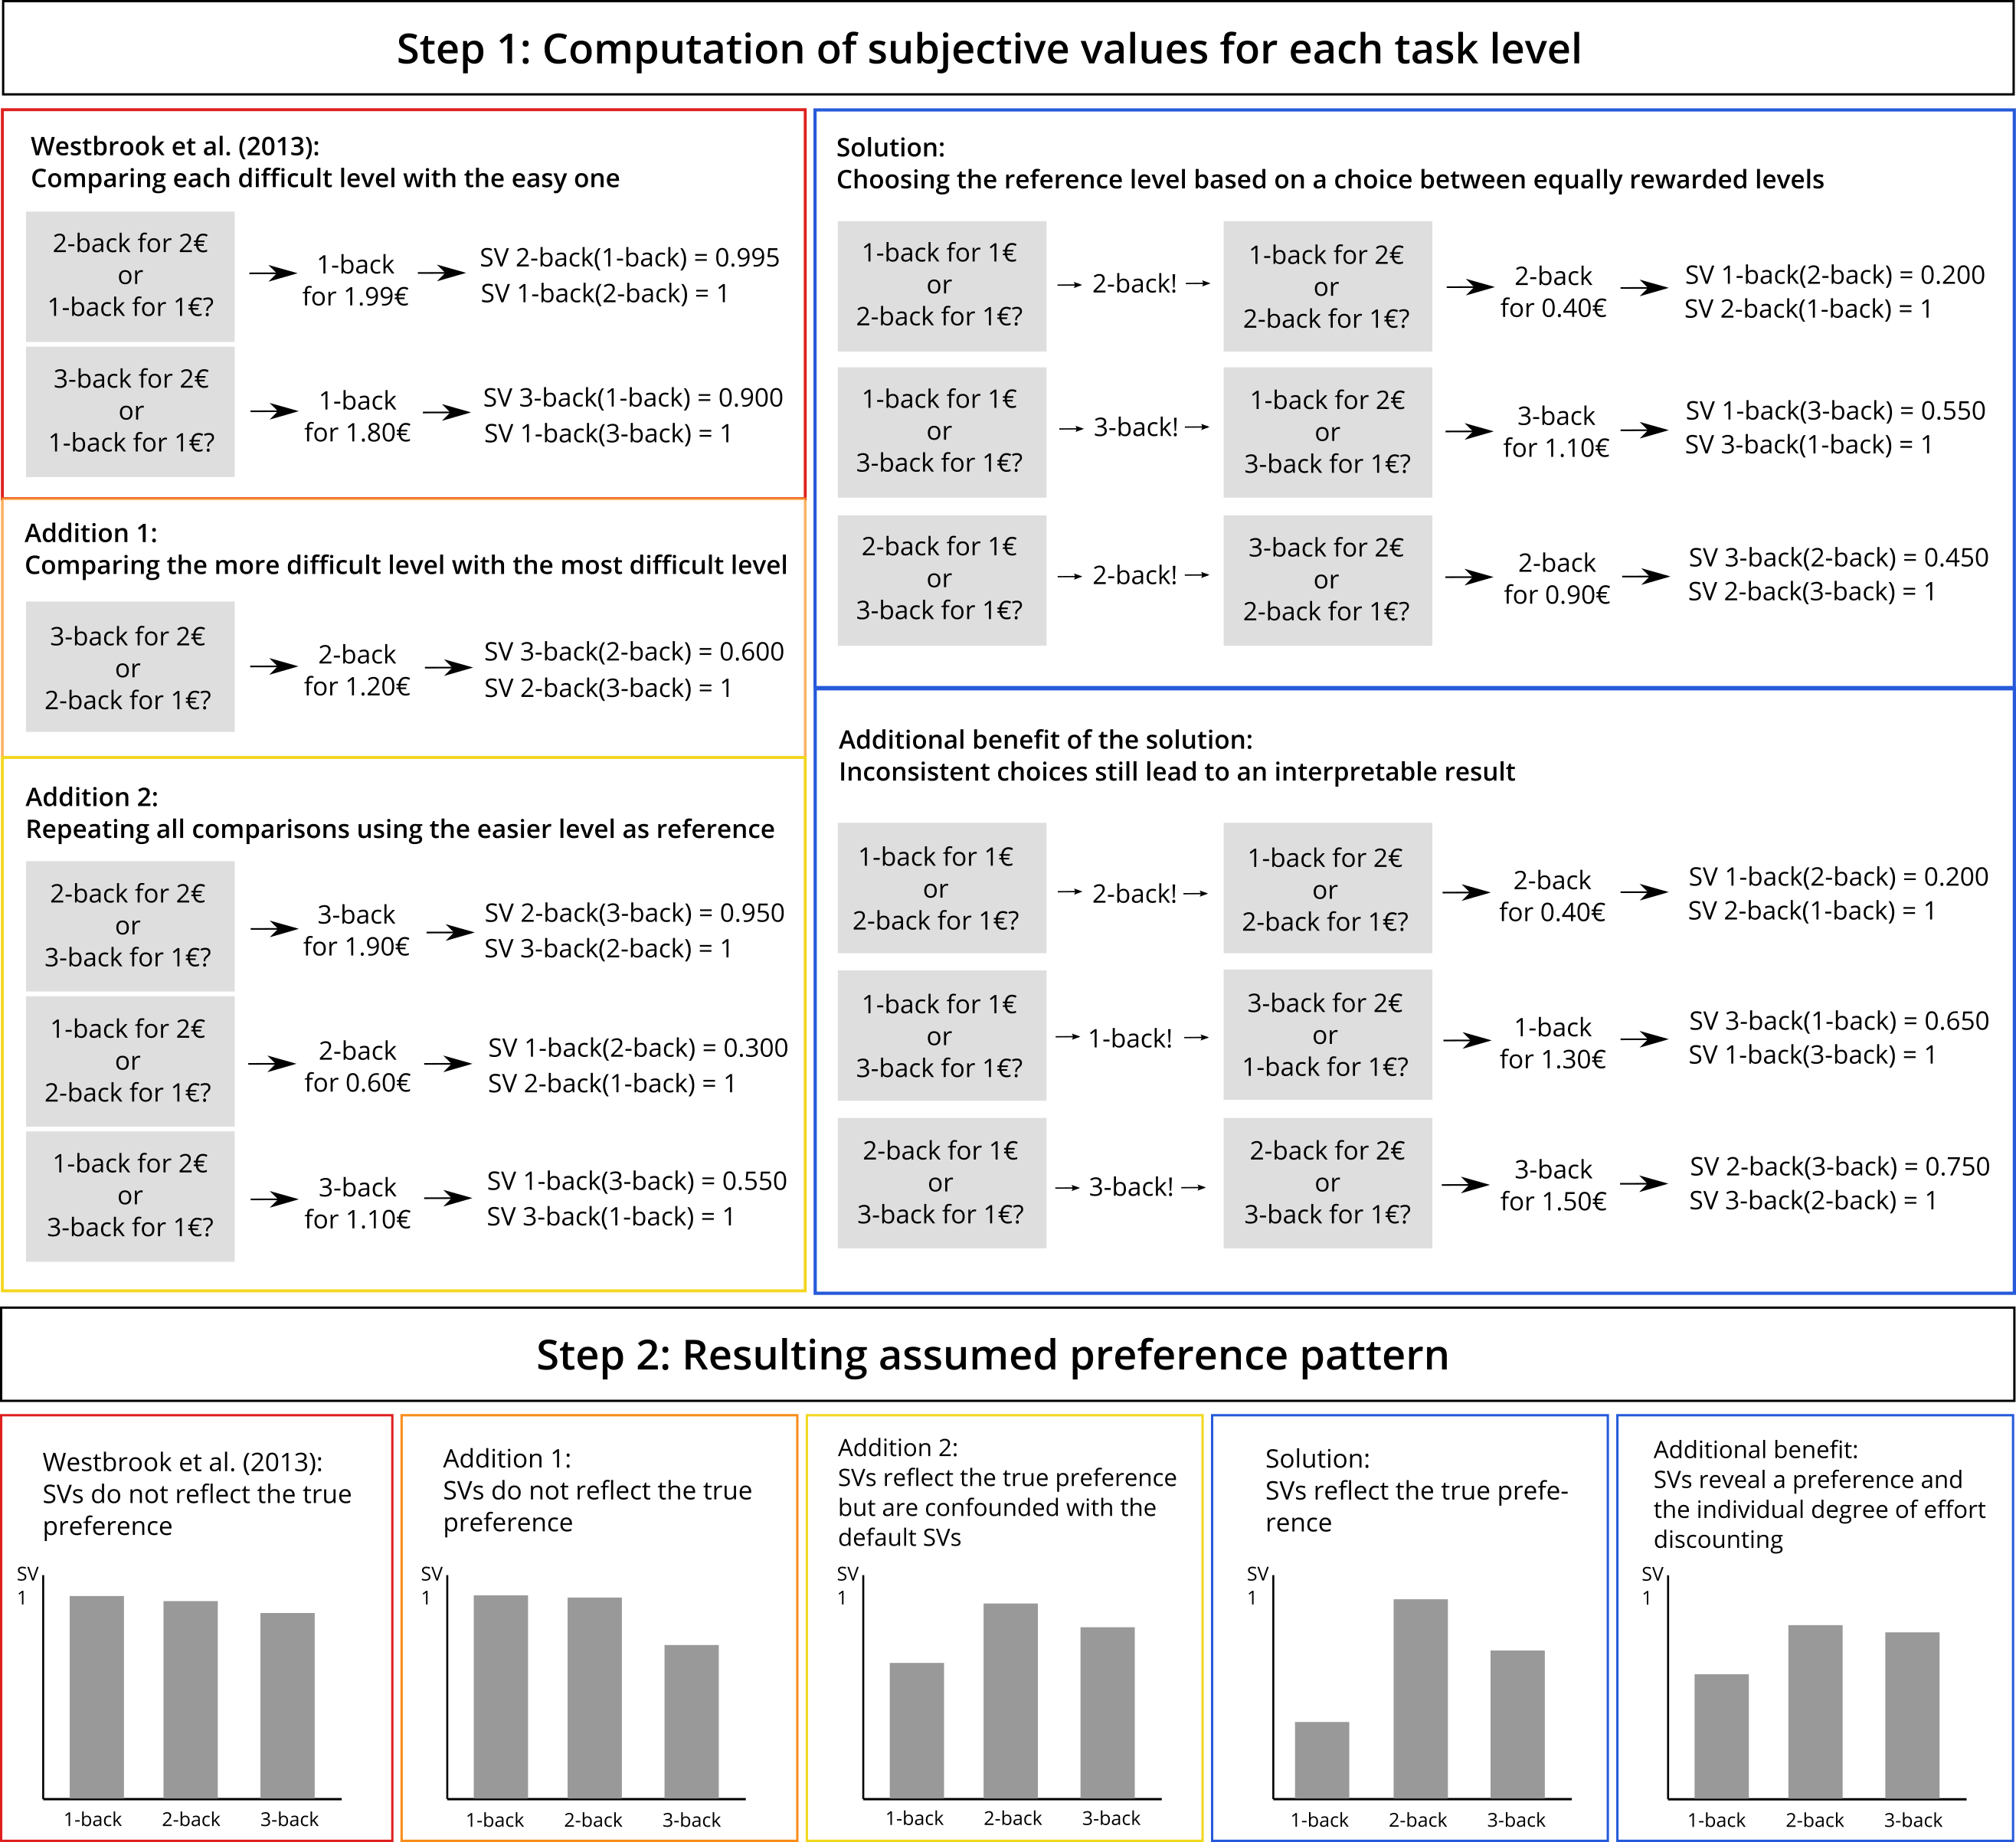
\includegraphics[width=\textwidth]{../../Inkscape Figures/Paradigm_Scheme} \caption{An example for subjective values for an $n$-back task with three levels, returned by different modifications of the COG-ED paradigm for a hypothetical participant with the true preference 2-back > 3-back > 1-back. The grey boxes are the choice options shown to the participant. The participant's final reward value of the flexible level is displayed after the first arrow. The resulting subjective value of each level is displayed after the second arrow, in the notation "SV 3-back(1-back)" for the subjective value of 3-back when 1-back is the other choice. The Solution and Additional Benefit panel follow the same logic, but are preceded by a choice between equal rewards, and the participant's first choice indicated by an exclamation mark. Figure available at osf.io/vnj8x/, under a CC-BY-4.0 license.}\label{fig:cadparadigm}
\end{figure}

\begin{figure}[H]
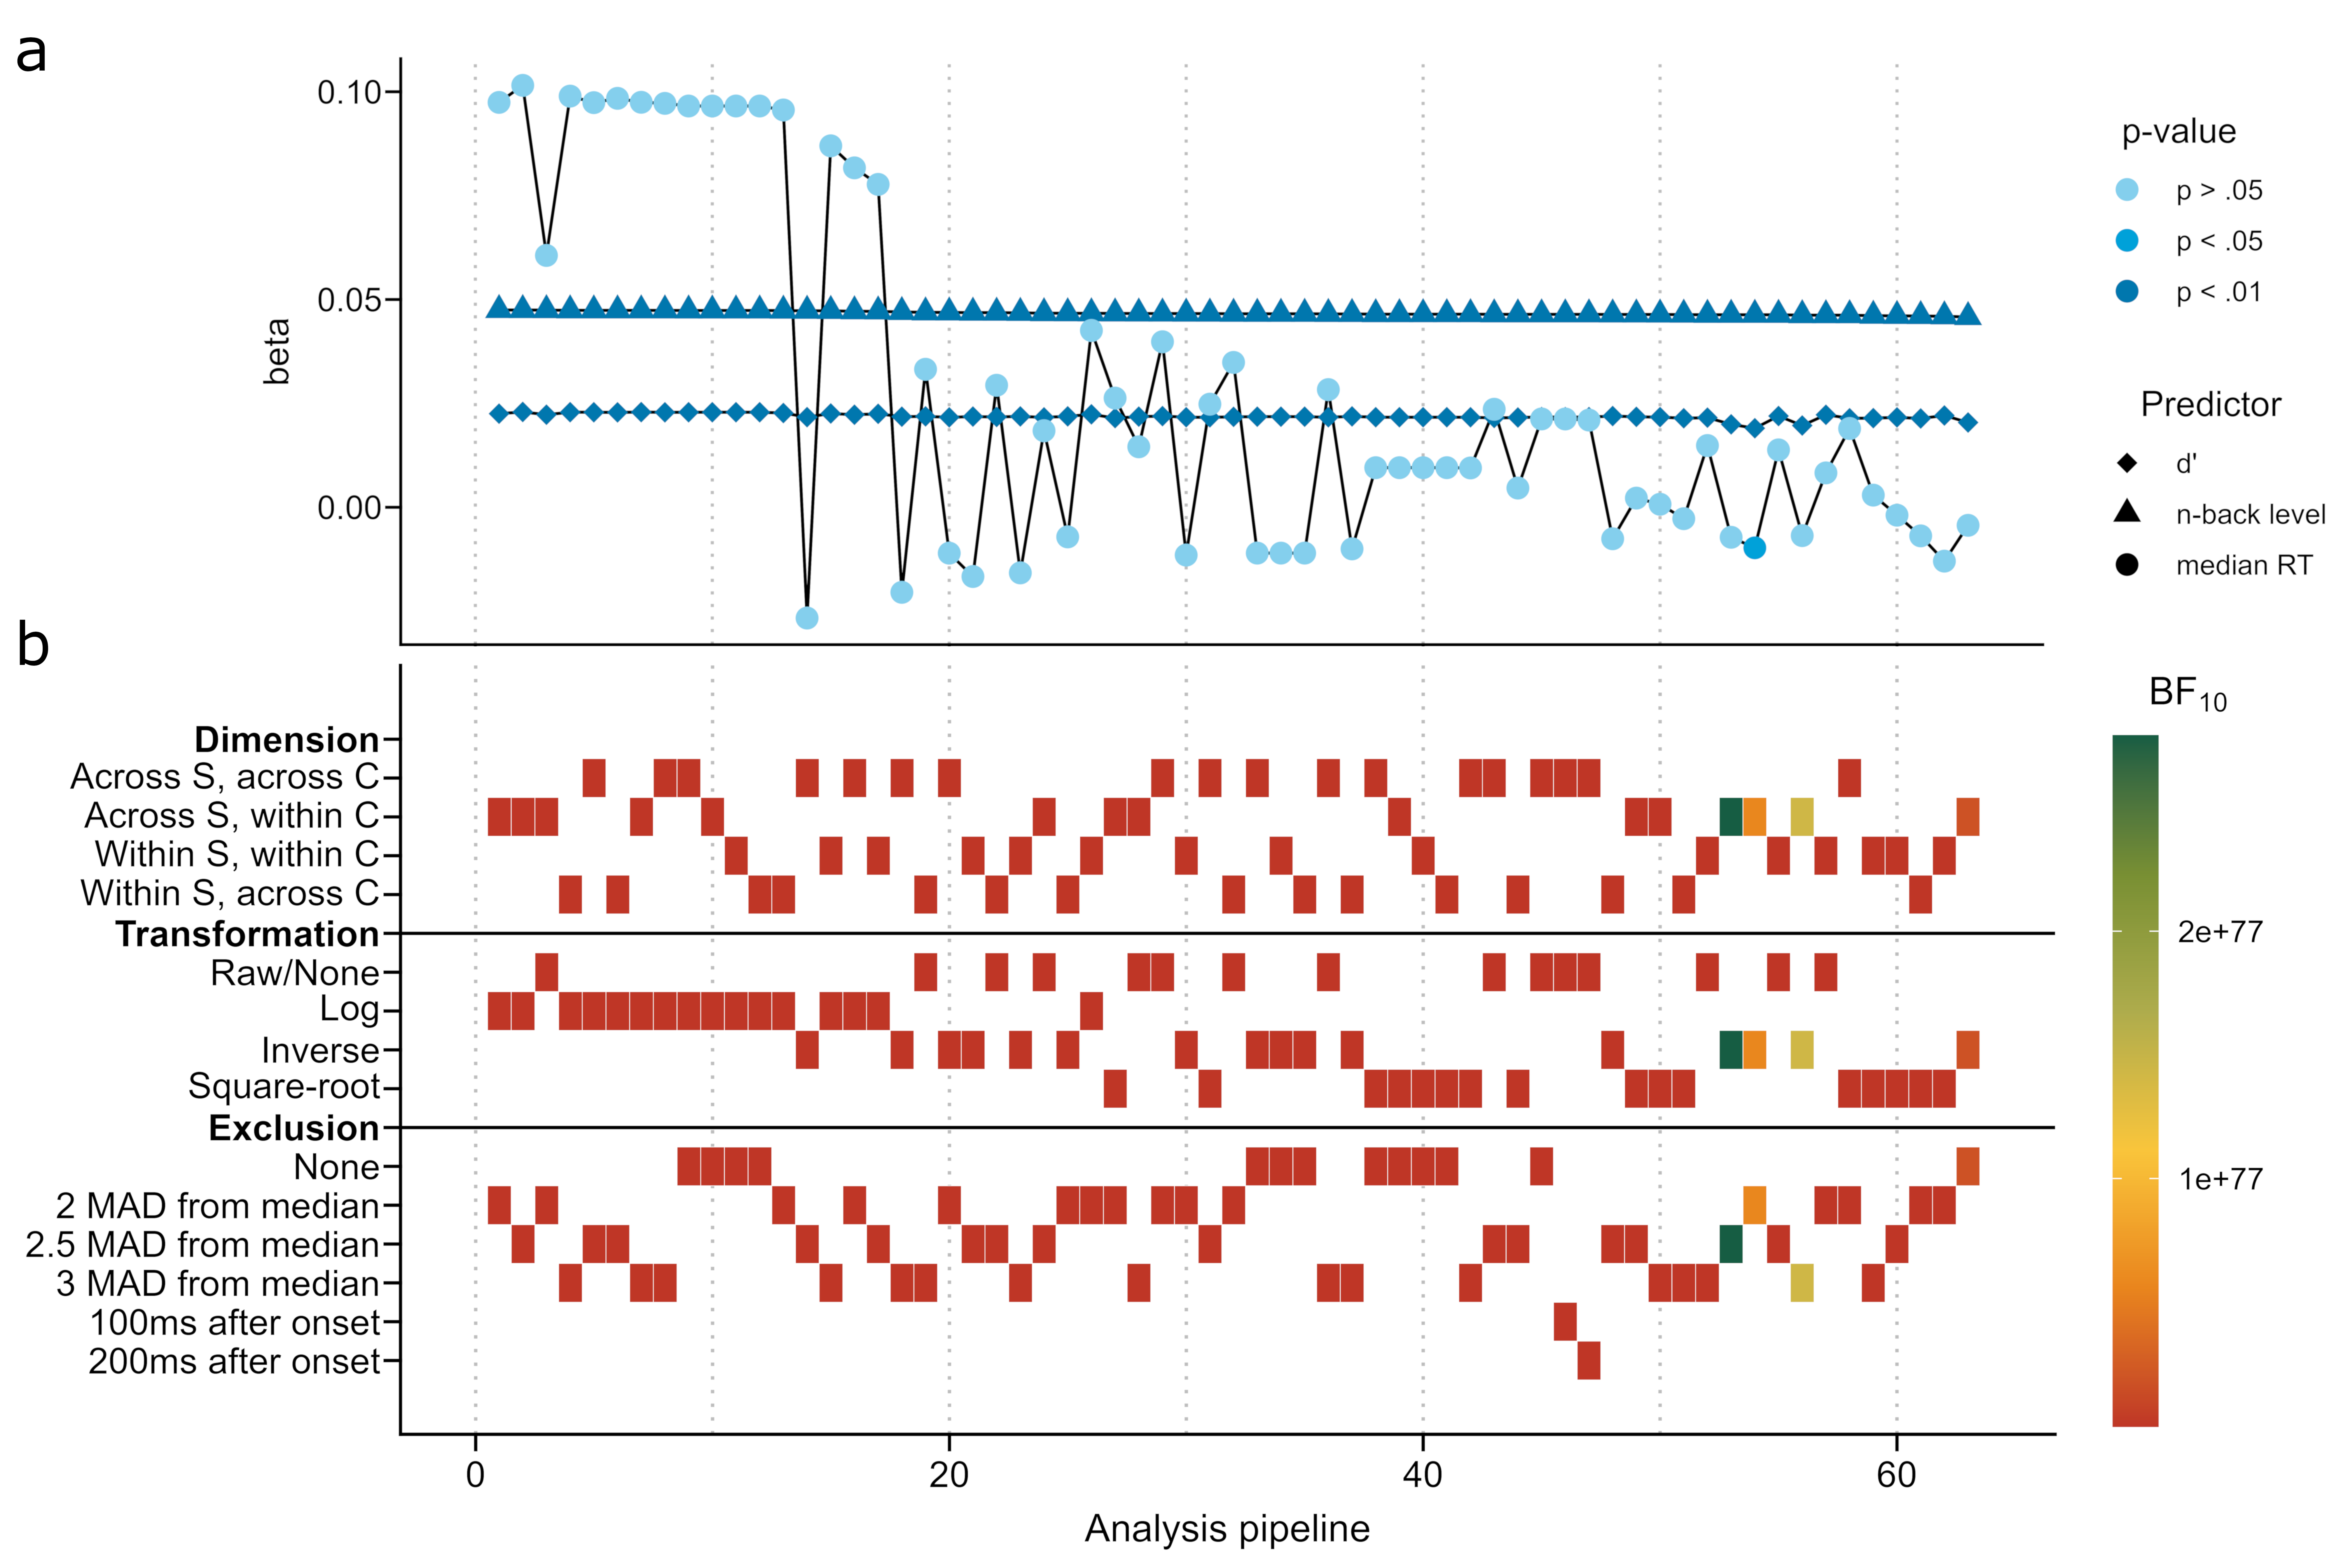
\includegraphics[width=\textwidth]{Figures/sca-plot} \caption{Results of the multi level model for each of the 63 preprocessing pipelines. Drawing a vertical through both panels indicates the type of preprocessing (panel b) of the pipeline and the resulting beta estimates of the three predictors in the model (panel a). The colourbar in panel b indicates the BF10 of each multi level model compared to a model in which the n-back level has no effect. The pipelines in both panels are sorted left to right in descending order of the magnitude of the beta estimate of the predictor n-back level. Figure available at osf.io/vnj8x/, under a CC-BY-4.0 license.}\label{fig:sca-plot}
\end{figure}

\begin{figure}[H]
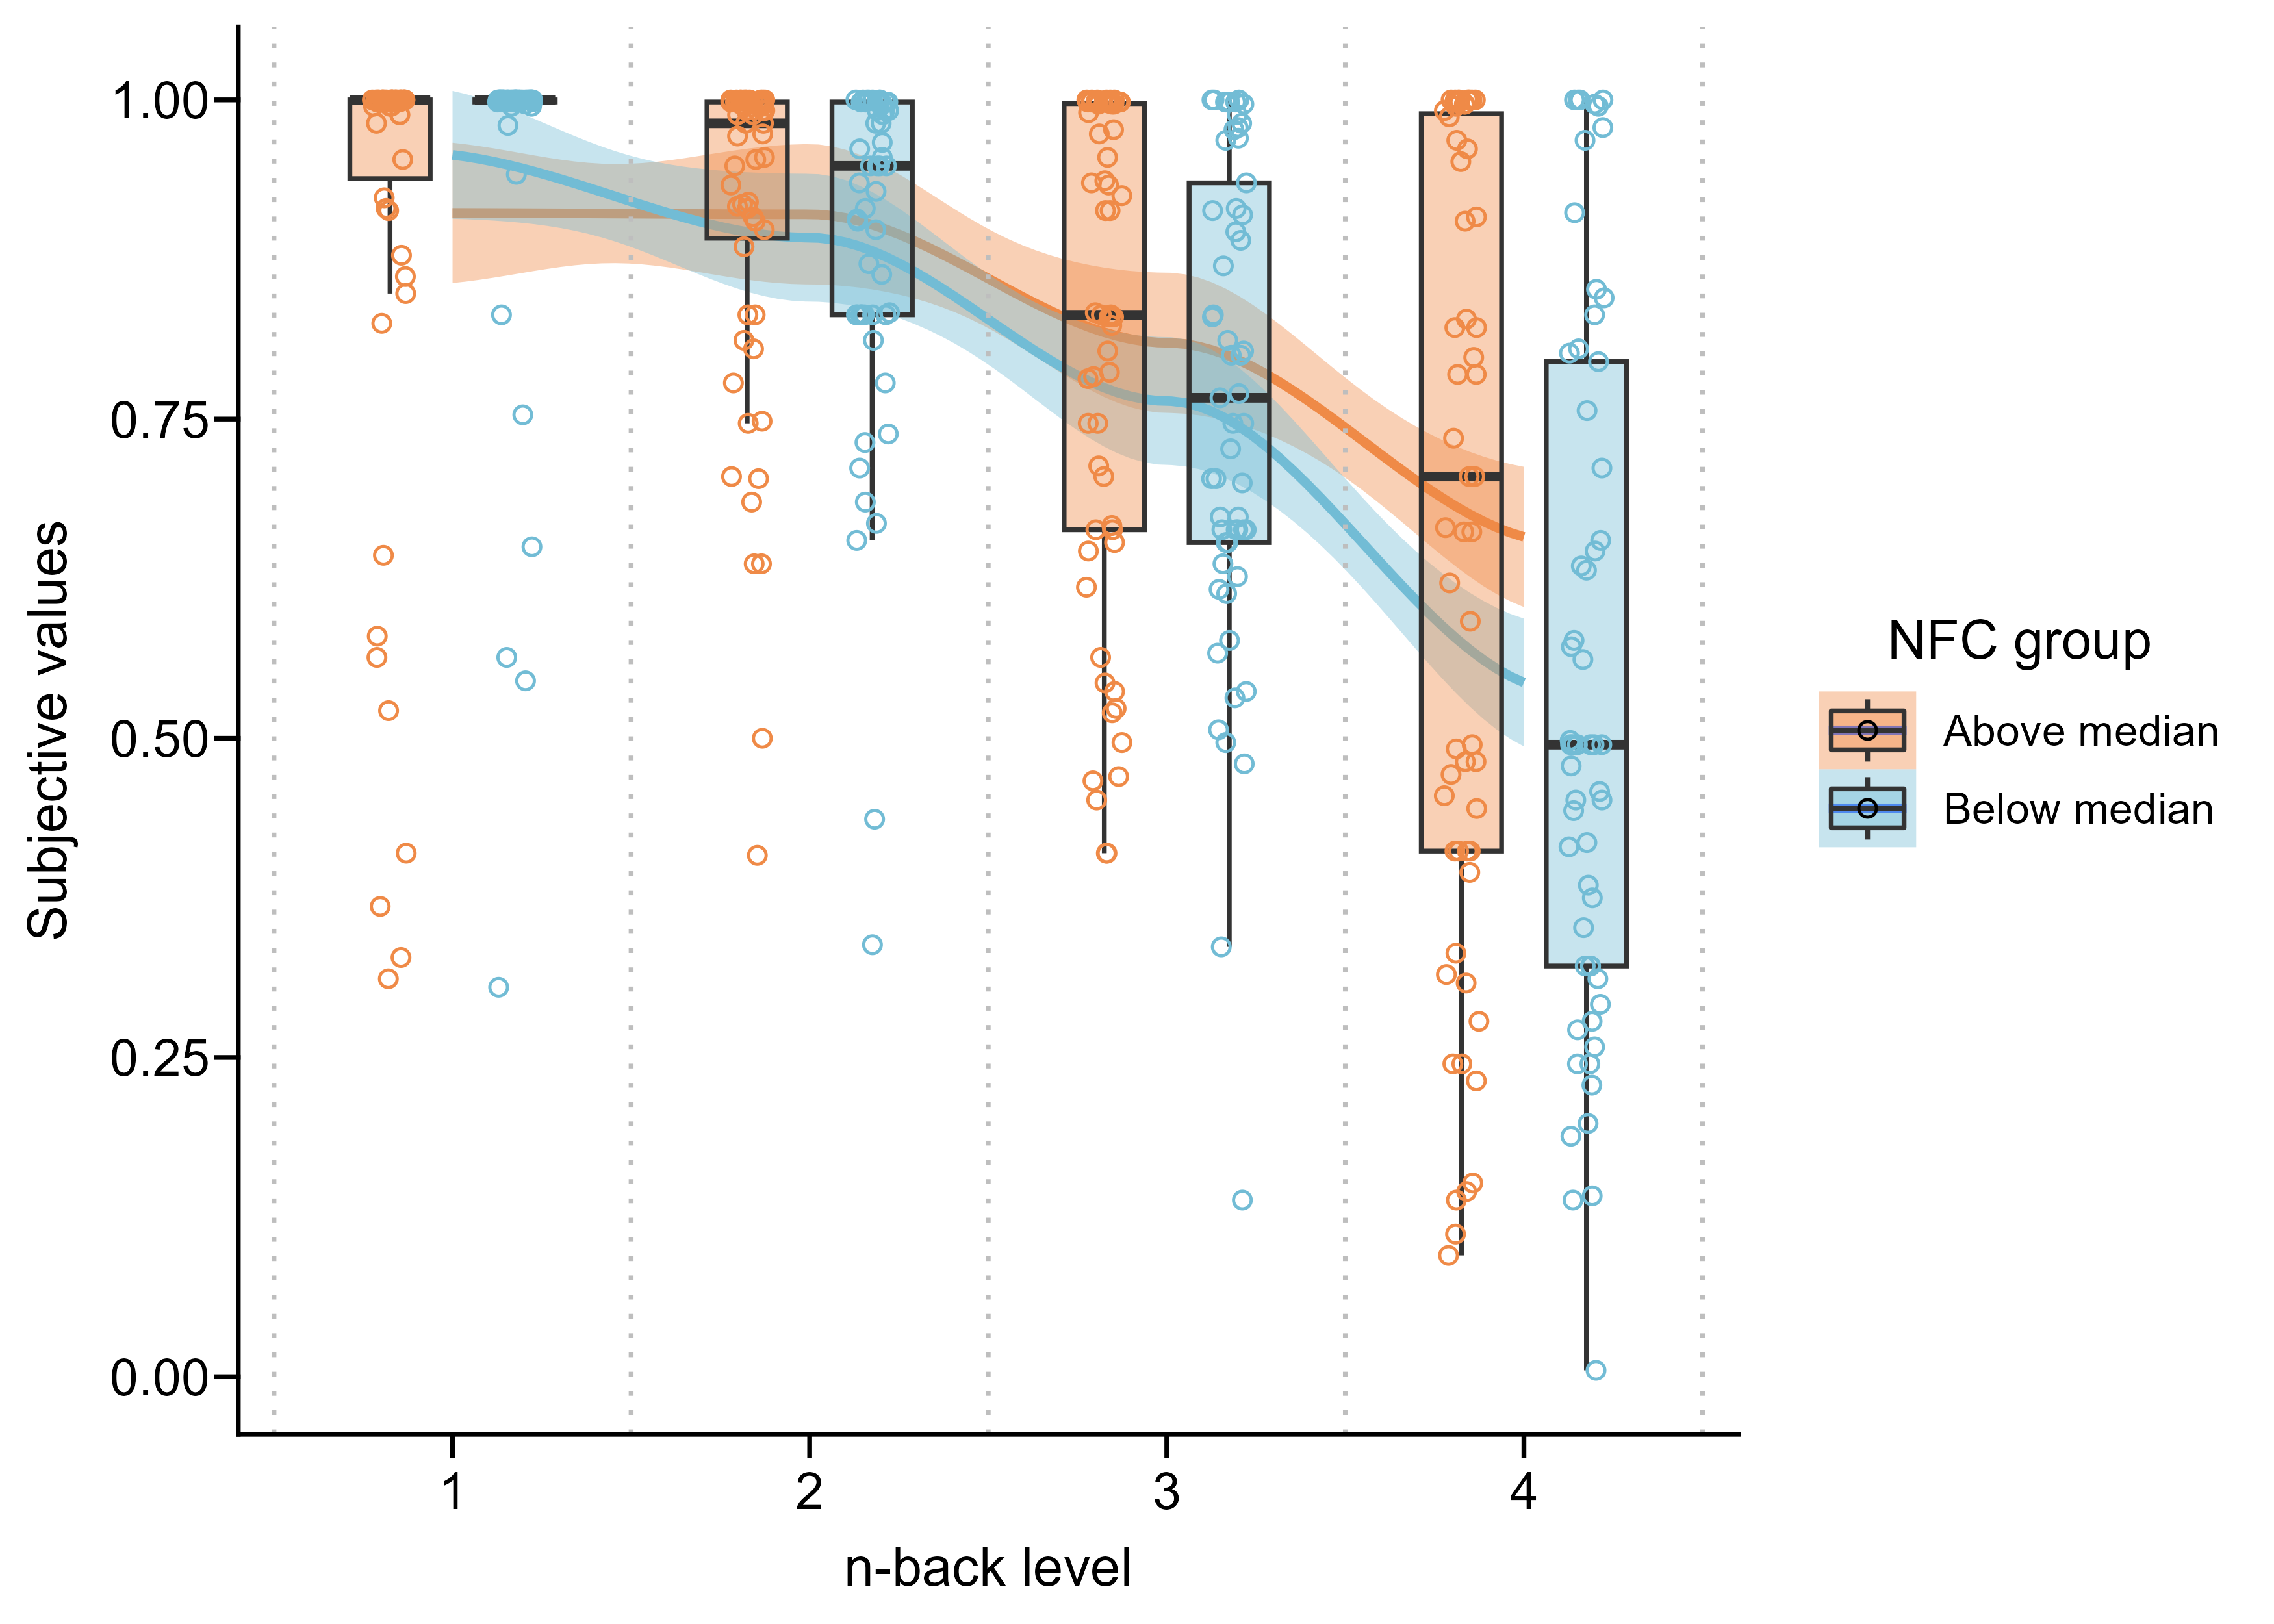
\includegraphics[width=\textwidth]{Figures/nfcgroups-sv} \caption{Subjective values per n-back level for participants with Need for Cognition (NFC) scores above and below the median. $N=116$. The scatter has a horizontal jitter of 0.2. Smoothing of conditional means with Loess method. Figure available at osf.io/vnj8x/, under a CC-BY-4.0 license.}\label{fig:nfcgroups-sv}
\end{figure}

\begin{figure}[H]
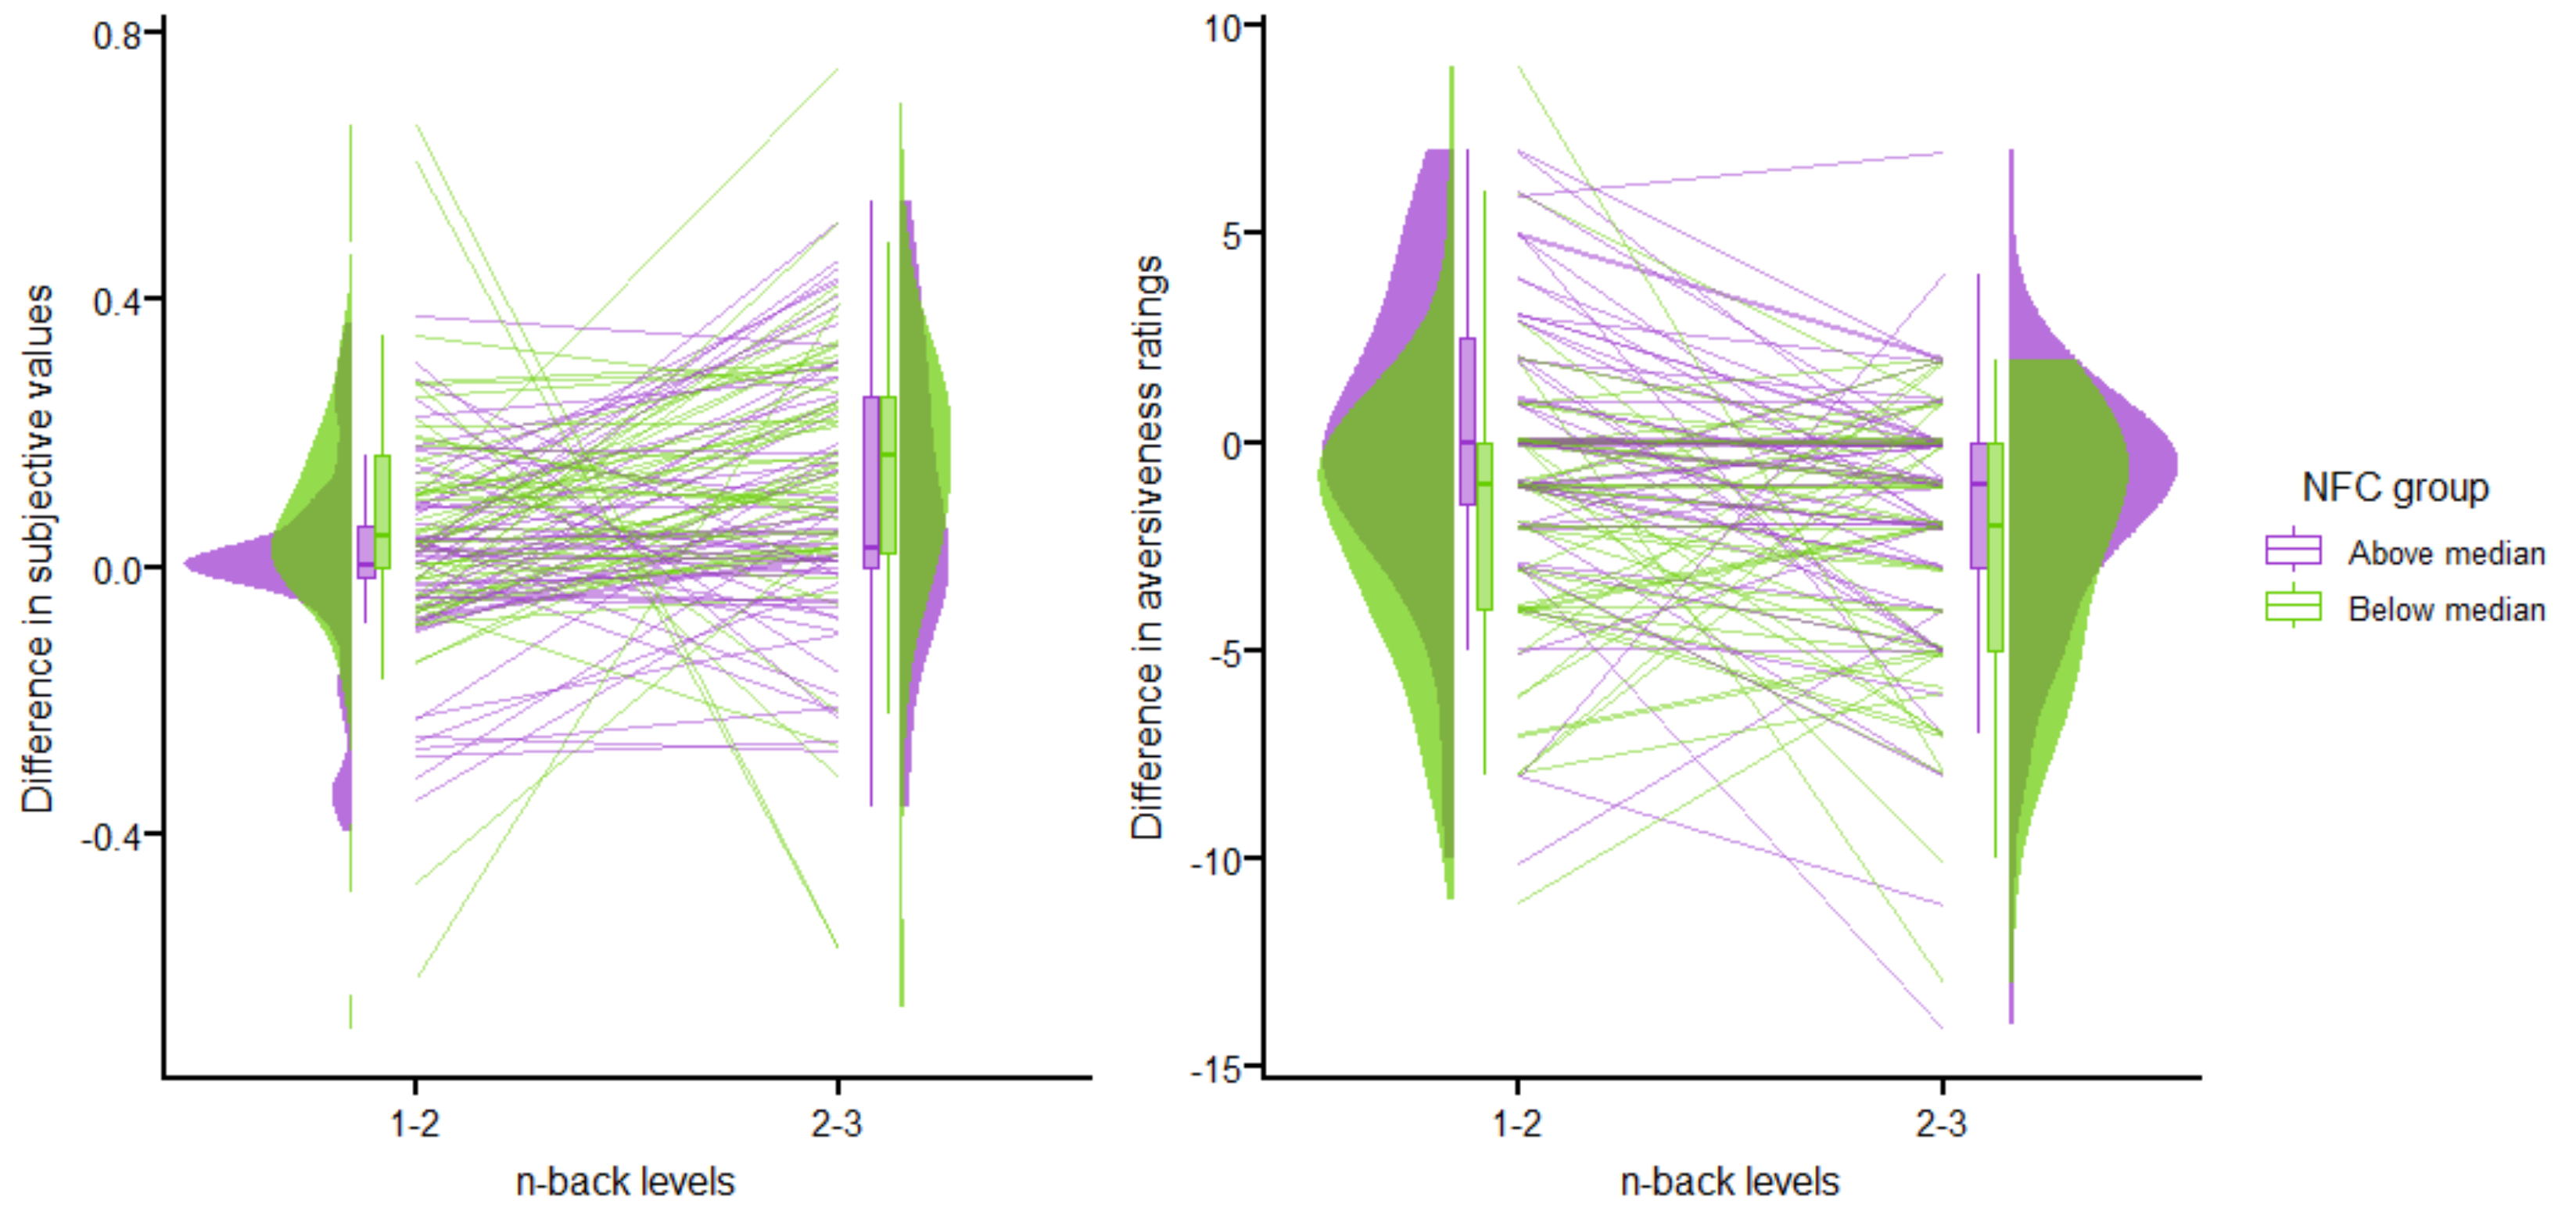
\includegraphics[width=\textwidth]{Figures/h3ac-plot} \caption{Difference scores for subjective values (a) and aversiveness ratings (b) when subtracting 2- from 1-back and 3- from 2-back. Horizontal lines of the boxplots represent the median per group, whiskers represent 1.5 interquartile ranges. NFC = Need for Cognition score. $N=116$. Figure available at osf.io/vnj8x/, under a CC-BY-4.0 license.}\label{fig:h3ac-plot}
\end{figure}

\begin{figure}[H]
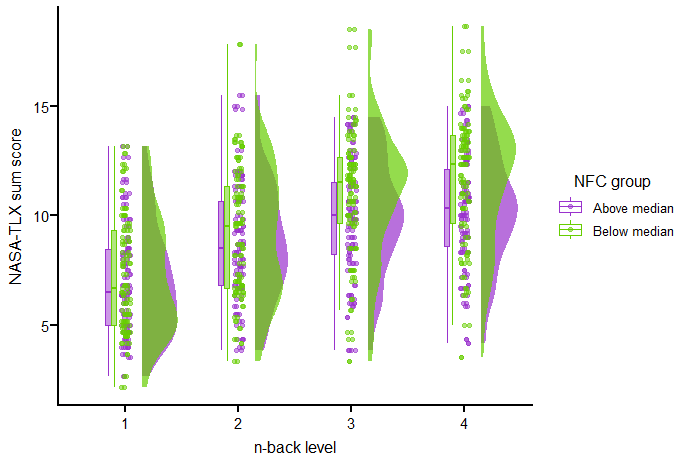
\includegraphics[width=\textwidth]{Figures/h3b-plot} \caption{NASA-TLX sum scores for each $n$-back level. Colours indicate Need for Cognition (NFC) score above or below the median. $N=116$. Figure available at osf.io/vnj8x/, under a CC-BY-4.0 license.}\label{fig:h3b-plot}
\end{figure}


\end{document}
